%% abtex2-modelo-trabalho-academico.tex, v-1.9.6 laurocesar
%% Copyright 2012-2016 by abnTeX2 group at http://www.abntex.net.br/ 
%%
%% This work may be distributed and/or modified under the
%% conditions of the LaTeX Project Public License, either version 1.3
%% of this license or (at your option) any later version.
%% The latest version of this license is in
%%   http://www.latex-project.org/lppl.txt
%% and version 1.3 or later is part of all distributions of LaTeX
%% version 2005/12/01 or later.
%%
%% This work has the LPPL maintenance status `maintained'.
%% 
%% The Current Maintainer of this work is the abnTeX2 team, led
%% by Lauro César Araujo. Further information are available on 
%% http://www.abntex.net.br/
%%
%% This work consists of the files abntex2-modelo-trabalho-academico.tex,
%% abntex2-modelo-include-comandos and abntex2-modelo-references.bib
%%

% ------------------------------------------------------------------------
% ------------------------------------------------------------------------
% abnTeX2: Modelo de Trabalho Academico (tese de doutorado, dissertacao de
% mestrado e trabalhos monograficos em geral) em conformidade com 
% ABNT NBR 14724:2011: Informacao e documentacao - Trabalhos academicos -
% Apresentacao
% ------------------------------------------------------------------------
% ------------------------------------------------------------------------

\documentclass[
	% -- opções da classe memoir --
	12pt,				% tamanho da fonte
	openany,			% capítulos começam em qualquer pagina (não insere página vazia caso preciso)
	twoside,			% para impressão em recto e verso. Oposto a oneside
	a4paper,			% tamanho do papel. 
	% -- opções da classe abntex2 --
	%chapter=TITLE,		% títulos de capítulos convertidos em letras maiúsculas
	%section=TITLE,		% títulos de seções convertidos em letras maiúsculas
	%subsection=TITLE,	% títulos de subseções convertidos em letras maiúsculas
	%subsubsection=TITLE,% títulos de subsubseções convertidos em letras maiúsculas
	% -- opções do pacote babel --
	english,			% idioma adicional para hifenização
	french,				% idioma adicional para hifenização
	spanish,			% idioma adicional para hifenização
	brazil				% o último idioma é o principal do documento
	]{abntex2}

% ---
% Pacotes básicos 
% ---
\usepackage{lmodern}			% Usa a fonte Latin Modern			
\usepackage[T1]{fontenc}		% Selecao de codigos de fonte.
\usepackage[utf8]{inputenc}		% Codificacao do documento (conversão automática dos acentos)
\usepackage{lastpage}			% Usado pela Ficha catalográfica
\usepackage{indentfirst}		% Indenta o primeiro parágrafo de cada seção.
\usepackage{color}				% Controle das cores
\usepackage{graphicx}			% Inclusão de gráficos
\usepackage{microtype} 			% para melhorias de justificação
\usepackage{mathtools}                         %Paradas matemáticas
\usepackage{listings}                              %Listagem de código
\usepackage{longtable}                          %Tabelas
\lstset{basicstyle=\tiny}
% ---
		
% ---
% Pacotes adicionais, usados apenas no âmbito do Modelo Canônico do abnteX2
% ---
\usepackage{lipsum}				% para geração de dummy text
% ---

% ---
% Pacotes de citações
% ---
\usepackage[brazilian,hyperpageref]{backref}	 % Paginas com as citações na bibl
\usepackage[alf]{abntex2cite}	% Citações padrão ABNT

% --- 
% CONFIGURAÇÕES DE PACOTES
% --- 

% ---
% Configurações do pacote backref
% Usado sem a opção hyperpageref de backref
\renewcommand{\backrefpagesname}{Citado na(s) página(s):~}
% Texto padrão antes do número das páginas
\renewcommand{\backref}{}
% Define os textos da citação
\renewcommand*{\backrefalt}[4]{
	\ifcase #1 %
		Nenhuma citação no texto.%
	\or
		Citado na página #2.%
	\else
		Citado #1 vezes nas páginas #2.%
	\fi}%
% ---

% ---
% Informações de dados para CAPA e FOLHA DE ROSTO
% ---
\titulo{ESTUDO DOS EFEITOS DO TÓRIO EM CONFIGURAÇÕES CRÍTICAS ORIENTADO PARA VERIFICAR OS DADOS NUCLEARES UTILIZADOS EM SIMULAÇÕES MONTE CARLO}
\autor{LUIZ FERNANDO BIANCHI DOS SANTOS}
\local{Brasil}
\data{Santo André, 7 de Maio de 2018}
\orientador{Prof. Dr. Pedro Carlos Russo Rossi}
\instituicao{%
  Universidade Federal do ABC -- UFABC
  \par
  Centro de Engenharia, Modelagem e Ciências Sociais Aplicadas -- CECS
  \par
 Graduação em Engenharia de Energia}
\tipotrabalho{Trabalho de Graduação}
% O preambulo deve conter o tipo do trabalho, o objetivo, 
% o nome da instituição e a área de concentração 
\preambulo{Trabalho de graduação, apresentado para a conclusão do curso de Graduação em Engenharia de Energia}
% ---


% ---
% Configurações de aparência do PDF final

% alterando o aspecto da cor azul
\definecolor{blue}{RGB}{41,5,195}

% informações do PDF
\makeatletter
\hypersetup{
     	%pagebackref=true,
		pdftitle={\@title}, 
		pdfauthor={\@author},
    	pdfsubject={\imprimirpreambulo},
	    pdfcreator={LaTeX with abnTeX2},
		pdfkeywords={abnt}{latex}{abntex}{abntex2}{trabalho acadêmico}, 
		colorlinks=true,       		% false: boxed links; true: colored links
    	linkcolor=blue,          	% color of internal links
    	citecolor=blue,        		% color of links to bibliography
    	filecolor=magenta,      		% color of file links
		urlcolor=blue,
		bookmarksdepth=4
}
\makeatother
% --- 

% --- 
% Espaçamentos entre linhas e parágrafos 
% --- 

% O tamanho do parágrafo é dado por:
\setlength{\parindent}{1.3cm}

% Controle do espaçamento entre um parágrafo e outro:
\setlength{\parskip}{0.2cm}  % tente também \onelineskip

% ---
% compila o indice
% ---
\makeindex
% ---

% ----
% Início do documento
% ----
\begin{document}

% Seleciona o idioma do documento (conforme pacotes do babel)
%\selectlanguage{english}
\selectlanguage{brazil}

% Retira espaço extra obsoleto entre as frases.
\frenchspacing 

% ----------------------------------------------------------
% ELEMENTOS PRÉ-TEXTUAIS
% ----------------------------------------------------------
% \pretextual

% ---
% Capa
% ---
\imprimircapa
% ---

% ---
% Folha de rosto
% (o * indica que haverá a ficha bibliográfica)
% ---
\imprimirfolhaderosto*
% ---

% ---
% Inserir a ficha bibliografica
% ---

% Isto é um exemplo de Ficha Catalográfica, ou ``Dados internacionais de
% catalogação-na-publicação''. Você pode utilizar este modelo como referência. 
% Porém, provavelmente a biblioteca da sua universidade lhe fornecerá um PDF
% com a ficha catalográfica definitiva após a defesa do trabalho. Quando estiver
% com o documento, salve-o como PDF no diretório do seu projeto e substitua todo
% o conteúdo de implementação deste arquivo pelo comando abaixo:
%
% \begin{fichacatalografica}
%     \includepdf{fig_ficha_catalografica.pdf}
% \end{fichacatalografica}

\begin{fichacatalografica}
	\sffamily
	\vspace*{\fill}					% Posição vertical
	\begin{center}					% Minipage Centralizado
	\fbox{\begin{minipage}[c][8cm]{13.5cm}		% Largura
	\small
	%\imprimirautor
	%Sobrenome, Nome do autor
	
	\hspace{0.5cm} \imprimirtitulo  / \imprimirautor. --
	\imprimirlocal, \imprimirdata-
	
	\hspace{0.5cm} \pageref{LastPage} p. : il. (algumas color.) ; 30 cm.\\
	
	\hspace{0.5cm} \imprimirorientadorRotulo~\imprimirorientador\\
	
	\hspace{0.5cm}
	\parbox[t]{\textwidth}{\imprimirtipotrabalho~--~\imprimirinstituicao.}\\
	
	\hspace{0.5cm}
		1. Tório.
		2. MCNP.
		2.Reatores Nucleares.
		I. Pedro Carlos Russo Rossi.
		II. Universidade Federal do ABC.
		III. Centro de Engenharia e Ciências Sociais Aplicadas.
		%IV. Estudos dos efeitos do Tório em configurações críticas orientado para verificar os dados nucleares utilizados em simulações Monte Carlo 			
	\end{minipage}}
	\end{center}
\end{fichacatalografica}
% ---

% ---
% Inserir errata
% ---
%\begin{errata}
%Elemento opcional da \citeonline[4.2.1.2]{NBR14724:2011}. Exemplo:

%\vspace{\onelineskip}

%FERRIGNO, C. R. A. \textbf{Tratamento de neoplasias ósseas apendiculares com
%reimplantação de enxerto ósseo autólogo autoclavado associado ao plasma
%rico em plaquetas}: estudo crítico na cirurgia de preservação de membro em
%cães. 2011. 128 f. Tese (Livre-Docência) - Faculdade de Medicina Veterinária e
%Zootecnia, Universidade de São Paulo, São Paulo, 2011.

%\begin{table}[htb]
%\center
%\footnotesize
%\begin{tabular}{|p{1.4cm}|p{1cm}|p{3cm}|p{3cm}|}
%  \hline
%   \textbf{Folha} & \textbf{Linha}  & \textbf{Onde se lê}  & \textbf{Leia-se}  \\
%   \hline
%   1 & 10 & auto-conclavo & autoconclavo\\
%  \hline
%\end{tabular}
%\end{table}

%\end{errata}
% ---

% ---
% Inserir folha de aprovação
% ---

% Isto é um exemplo de Folha de aprovação, elemento obrigatório da NBR
% 14724/2011 (seção 4.2.1.3). Você pode utilizar este modelo até a aprovação
% do trabalho. Após isso, substitua todo o conteúdo deste arquivo por uma
% imagem da página assinada pela banca com o comando abaixo:
%
% \includepdf{folhadeaprovacao_final.pdf}
%
\begin{folhadeaprovacao}

  \begin{center}
    {\ABNTEXchapterfont\large\imprimirautor}

    \vspace*{\fill}\vspace*{\fill}
    \begin{center}
      \ABNTEXchapterfont\bfseries\Large\imprimirtitulo
    \end{center}
    \vspace*{\fill}
    
    \hspace{.45\textwidth}
    \begin{minipage}{.5\textwidth}
        \imprimirpreambulo
    \end{minipage}%
    \vspace*{\fill}
   \end{center}
        
   Trabalho aprovado. \imprimirlocal, 10 de Maio de 2018:

   \assinatura{\textbf{\imprimirorientador} \\ Orientador} 
   \assinatura{\textbf{Professor} \\ Convidado 1}
   \assinatura{\textbf{Professor} \\ Convidado 2}
   %\assinatura{\textbf{Professor} \\ Convidado 3}
   %\assinatura{\textbf{Professor} \\ Convidado 4}
      
   \begin{center}
    \vspace*{0.5cm}
    {\large\imprimirlocal}
    \par
    {\large\imprimirdata}
    \vspace*{1cm}
  \end{center}
  
\end{folhadeaprovacao}
% ---

% ---
% Dedicatória
% ---
\begin{dedicatoria}
   \vspace*{\fill}
   \centering
   \noindent
   \textit{ Este trabalho é dedicado aos meus pais, padrinhos e irmãos, que \\
   me apoiaram na longa jornada da graduação e à minha noiva que \\
   , muitas vezes, redefiniu o significado de paciência.} \vspace*{\fill}
\end{dedicatoria}
% ---

% ---
% Agradecimentos
% ---
\begin{agradecimentos}

Os agradecimentos vão para os Professores Doutores da Universidade Federal do ABC Pedro Carlos Russo Rossi e João Manoel Losada Moreira, que viabilizaram com grande esforço a execução deste trabalho. Principalmente o professor Pedro, fornecendo apoio até mesmo em situações de logística complicada. 

Além destes, faz juz ao agradecimento o aluno Vinícius Nery de Araújo Miranda, que prestou auxílio nas nuances do código em LaTeX e em diversos momentos durante o desenvolvimento do trabalho.

Sem o ensaio proposto pelo Professor João em seu artigo de 1998 a definição de alguns dos aspectos deste trabalho se tornaria muito mais demorada.

\end{agradecimentos}
% ---

% ---
% Epígrafe
% ---
\begin{epigrafe}
    \vspace*{\fill}
	\begin{flushright}
		\textit{``Em algum lugar, algo incrível \\ está esperando para ser descoberto.
		(Carl Sagan)}
	\end{flushright}
\end{epigrafe}
% ---

% ---
% RESUMOS
% ---

% resumo em português
\setlength{\absparsep}{18pt} % ajusta o espaçamento dos parágrafos do resumo
\begin{resumo}
A utilização de combustíveis a base de tório em reatores nucleares é a muito tempo cogitada como alternativa tecnológica para o desenvolvimento de reatores nucleares, porém, incertezas surgem no projeto destes sistemas devido a possíveis inconsistências que podem existir nos dados nucleares. Tendo em vista as largas reservas de Tório localizadas no território brasileiro, torna-se interessante explorar a possibilidade de utilizar este elemento como um componente base nos combustíveis nucleares. Enquanto a possibilidade do uso de tório em reatores já é conhecida, ainda é necessário que seja investido tempo e capital no desenvolvimento da tecnologia. Antes de realizar experimentos com varetas de Óxido deTório é inteligente que sejam analisados os resultados obtidos em simulações computacionais. O presente trabalho atende esta necessidade proponto duas configurações críticas utilizando varetas contendo Óxido de Tório para o reator IPEN/MB-01. Os resultados deste trabalho poderão ser comparados com resultados de um ensaio real para averiguar a confiabilidade dos dados de secção de choque disponíveis para o Tório. 

 \textbf{Palavras-chave}: Tório. MCNP. Reatores Nucleares. Reatores de Óxido Misto.
\end{resumo}

% resumo em inglês
\begin{resumo}[Abstract]
 \begin{otherlanguage*}{english}
   The use of Thorium based fuels in nuclear reactors has been seen as an technological alternative to the development of nuclear reactors, however, ucertainties arise in the project of these systems regarding the possibilty of problems that might exist in the nuclear data. Because of the large Thorium reserves located in the brazilian territory, it becomes interesting to explore the possibility of utilizing this element as a base component for nuclear fuels. Even tough the possibility to use Thorium in reactors is a well known fact, it is still necessary to invest some time and money in the development of the tecnology. Before the realization of experiments with Thorium Oxide rods it is smart to analize the results obtained in computational simulations; the present paper sees trough this need by proposing two critical configurations containing Thorium Oxide rods to the IPEN/MB-01 reactor. The results of this work may be compared to a real case scenario to ascertain the reliability of the cross section data avalaible for Thorium.

   \vspace{\onelineskip}
 
   \noindent 
   \textbf{Keywords}:Thorium. MCNP. Nuclear Reactors. Mixed Oxide Reactors.
 \end{otherlanguage*}
\end{resumo}

% ---
% inserir lista de ilustrações
% ---
\pdfbookmark[0]{\listfigurename}{lof}
\listoffigures*
\cleardoublepage
% ---

% ---
% inserir lista de tabelas
% ---
\pdfbookmark[0]{\listtablename}{lot}
\listoftables*
\cleardoublepage
% ---

% ---
% inserir lista de abreviaturas e siglas
% ---
\begin{siglas}
  \item[EPE] Empresa de Pesquisa Energética
  \item[IDH] Índice de Desenvolvimento Humano
  \item[IPEN] Instituto de Pesquisas Energéticas Nucleares 
  \item[IPEN/MB-01] Reator nuclear do IPEN, \emph{mock-up} do submarino nuclear brasileiro
  \item[HEU] \emph{Highly Enriched Uranium} - Urânio Altamente Enriquecido
  \item[IAEA] \emph{International Atomic Energi Assotiation} - Associação Internacional de Energia Nuclear
  \item[MCNP] \emph{Monte Carlo N-Particle} -  Monte Carlo Partícula N
  \item[LANL] \emph{Los Alamos National Lab} - Laboratório Nacional de Los Alamos 
  \item[MCNPX] Código do tipo MCNP de criação do LANL  
  \item[ENDF] \emph{Evaluated Nuclear Data File} - Arquivo de Dado Nuclear Avaliado 
  \item[ASTM] \emph{American Society for Testing and Materials} - Sociedade Americana para Testes e Materiais
  \item[AISI] \emph{American Iron and Steel Institute} - Instituto Americano de Ferro e Aço
\end{siglas}
% ---

% ---
% inserir lista de símbolos
% ---
%\begin{simbolos}
%  \item[$ \Gamma $] Letra grega Gama
%  \item[$ \Lambda $] Lambda
%  \item[$ \zeta $] Letra grega minúscula zeta
%  \item[$ \in $] Pertence
%\end{simbolos}
% ---

% ---
% inserir o sumario
% ---
\pdfbookmark[0]{\contentsname}{toc}
\tableofcontents*
\cleardoublepage
% ---



% ----------------------------------------------------------
% ELEMENTOS TEXTUAIS
% ----------------------------------------------------------
\textual

% ----------------------------------------------------------
% Introdução
% ----------------------------------------------------------
\chapter*[Introdução]{Introdução}
\addcontentsline{toc}{chapter}{Introdução}
% ----------------------------------------------------------

Segundo o Anuário Estatístico de Demanda Energética, fornecido pela EPE (Empresa de Pesquisa Energética), a demanda energética do Brasil em 2015 cresceu 10\% quando comparada à demanda energética de 2010; o consumo atual per capta, segundo a mesma fonte, aumentou de 2,37kWh/Ano para 2,63kWh/Ano, um aumento de 10,9\% em 5 anos\cite{11anuario}. Se compararmos estes dados com os de países com maior IDH, perceberemos que o consumo de energia no Brasil ainda está aquém do esperado, é imprescindível considerar este crescimento no planejamento energético de um país com as proporções territoriais do Brasil e nesse contexto a alternativa
nuclear se mostra como um forte candidata para atender às demandas futuras com grande grau de confiabilidade.

A expansão parque nuclear nacional ainda é um assunto delicado a ser abordado, principalmente devido a temas como acidentes severos, gerenciamento de rejeitos em toda cadeia de produção e competitividade econômica, entretanto, se observarmos benefícios como disponibilidade, constância de abastecimento e potência por metro quadrado ocupado em conjunto com os malefícios associados às outras alternativas energéticas \cite{15Impactos1}\cite{16Impactos2} vemos que o balanço entre riscos e benefícios da energia nuclear é bastante favorável. Protocolos de segurança internacionais tornaram os novos projetos de reatores mais seguros do que os projetos antigos. As tecnologias de estado da arte tornam a alternativa nuclear cada vez mais interessante. 

Outro fator estratégico que deve ser observado na avaliação da viabilidade da energia nuclear como parte sigificativa da matriz energética nacional é a disponibilidade de recursos. O Brasil possui tecnologia proprietária para enriquecimento de urânio e suas reservas naturais deste elemento estão dentro das três maiores do mundo\cite{17survey}, além disto, como será tratado neste trabalho, alguns elementos, com destaque para o Tório podem ser utilizados para gerar energia dentro de reatores nucleares com apenas pequenas alterações em suas configurações. 

Se formos capazes de dominar esta tecnologia e superarmos as barreiras, relacionadas intimamente ao preconceito e não a problemas factíveis, a energia nuclear pode permitir uma redução no custo operacional do setor industrial, culminando também em um acesso mais difundido da energia elétrica para toda a população brasileira. 

Este trabalho faz parte do início do processo de avaliação dos dados nucleares do Tório, através da proposição de dois arranjos críticos para o reator IPEN/MB-01, estes arranjos foram imaginados com a intenção de simplificar e barratear o processo de teste, utilizando varetas de fabricação simples e considerando o mínimo de varetas de teste possível no núcleo do reator.

% ----------------------------------------------------------
% Referenciais Teóricos
% ----------------------------------------------------------
% ---
% Capitulo de revisão de literatura
% ---
\chapter{Referenciais Teóricos}
% ---

% ----------------------------------------------------------
% SECÇÃO
% ----------------------------------------------------------
\section{Reatores Nucleares}

Um reator nuclear é uma máquina projetada para permitir indução e manutenção de uma cadeia de reações nucleares sucessivas. Uma reação nuclear é um tipo de reação onde ocorre a transmutação de um elemento em outro com subsequênte liberação de grandes quantidades de energia. Pode ser traçado um paralalelo entre uma reação nuclear e uma reação de combustão, pois o produto de uma reação nuclear gera o estopím (na forma de nêutrons) para as reações subsequentes nos elementos combustíveis ao redor do inicial, devido a estas semelhanças é comum utilizar os termos ``combustível nuclear'' para se referir aos elemento consumidos durante a reação nuclear e ``queima'' para se referir à reação nuclear.

Quando a fissão de um elemento gera novos nêutrons que causam novas fissões diz-se que foi iniciada uma reação em cadeia, este é o principio de funcionamento de um reator nuclear. As reações em cadeia podem ser estabelecidas em quantidades muito pequenas de material físsil, na situação chamada de massa crítica, entretanto, o consumo do combustível é muito rápido. O projeto do reator tem como objetivo a geração de uma situação de massa crítica em um modelo controlável e por um longo período de tempo. Para que seja feita utilização da energia proveniente das reações nucleares é necessário que seja possível controlar a taxa de reação e os chamados nêutrons lentos tem papel importante nesta função; a grosso modo uma reação nuclear pode gerar nêutrons dentro de um amplo espectro de energia e esta situação gera tempos de resposta que também variam dentro de um espectro. Para abrandaresta variação é comum o emprego de um moderador, como a água ou o
grafite, que reduz a energia dos nêutrons de maior energia (neutrôns rápidos) para os patamares dos nêutrons de menor energia (nêutrons lentos), a velocidade reduzida dos nêutrons lentos causa uma situação onde a resposta do reator assume fatores de tempo de ordens que permitem seu controle com segurança\cite{10fundamentos}. 

Outro fator importante é o controle do calor gerádo pelo denominado núcleo do reator, que deve ser removido para ser utilizado para geração de energia em um ciclo termodinâmico, para tal é empregado um refrigerante. O uso da água desmineralizada é comum mas como alguns produtos de fissão podem reagir com este refrigerante, normalmente utiliza-se um encapsulamento metálico ao redor do combustível para impedir o contato (i.e. varetas metálicas recheadas com Óxido de Urânio no IPEN/MB-01).

Em reatores do tipo PWR (\emph{Pressurized Water Reactor}-Reatores de Água Pressurizada), como é o caso dos reatores da Central Nuclear Almirante Álvaro Alberto: Angra 1, Angra 2 e o futuro reator de Angra 3, o calor é removido do núcleo utilizando a água em um sistema primário e, através de um trocador de calor, esta água presssurizada e aquecida troca calor com outra corrente de água à menor pressão, esta segunda corrente, por sua vez, passa por um Ciclo Rankine\cite{18termodinamica}; é transformada
em vapor superaquecido pela fonte quente e utilizada para movimentar uma turbina que movimenta um gerador elétrico, o vapor na saída da turbina é resfriado até a condensação e uma bomba realiza a reinjeção do fluído resfriado, fechando o ciclo. A utilização de dois sistemas separados isola a água utilizada para resfriar o núcleo do reator do sistema de geração de energia elétrica, este arranjo reduz o desgaste em alguns dos equipamentos mais caros do sistema (turbina e condensador) e garante maior segurança na operação. O sistema que será implementado em Angra 3 pode ser observado na figura ~\ref{PWR}.

\begin{figure}[htpb]
	\caption{\label{PWR} Esquemático do reator PWR de Angra 3.}
	\begin{center}
	    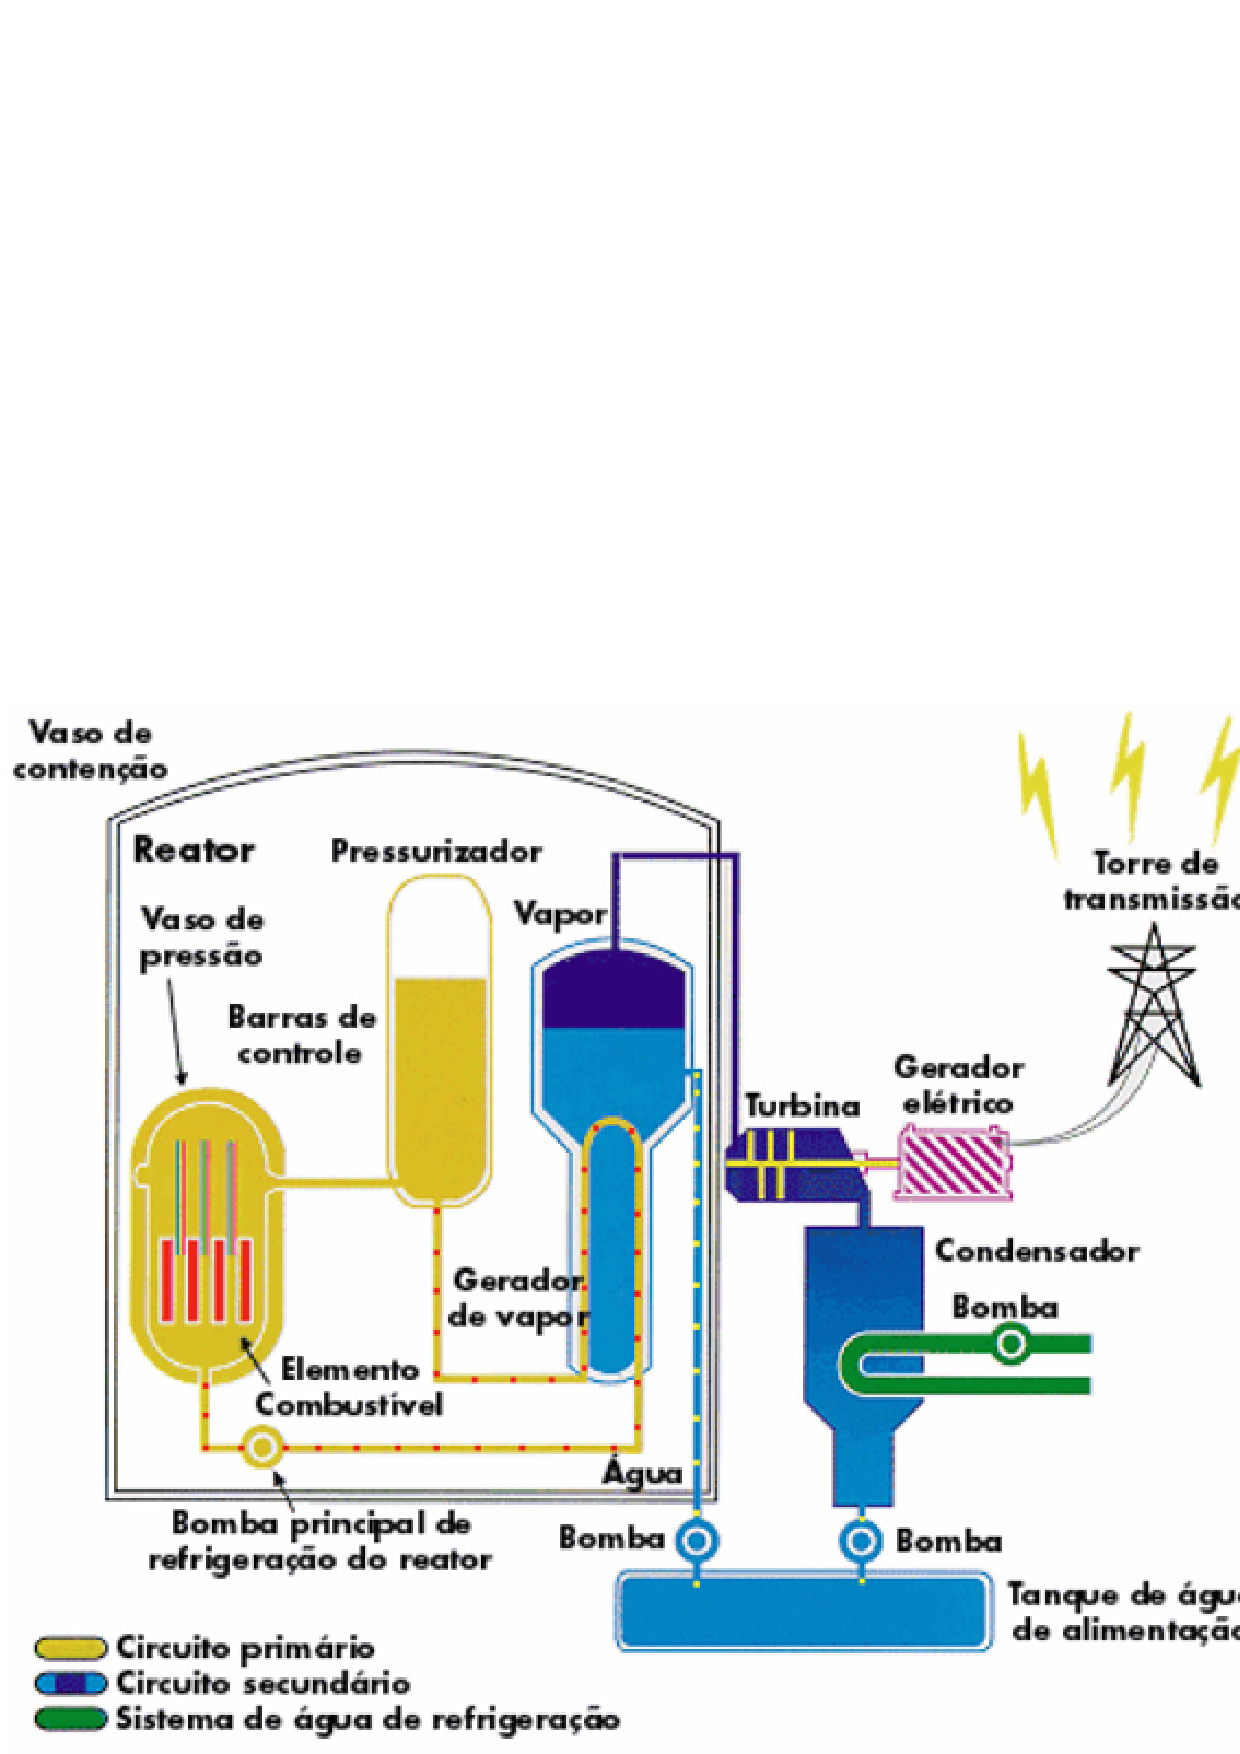
\includegraphics[scale=0.5]{figs/PWRAngra3.jpg}
	\end{center}
	\legend{Fonte: https://www.ipen.br/, acesso em 07/05/2018 às 20:00.}
\end{figure}

\section{Combustíveis Nucleares}

As reações de fissão nuclear ocorrem em uma grande quantidade de nuclídeos, nuclídeos que são passíveis de fissão nuclear em condições específicas são denominados fissionáveis, entretanto apenas alguns são apropriados para uso em reatores nucleares, a estes é atribuido o termo ``físseis''. É necessário que a reação de fissão tenha como produto dois ou mais nêutrons, além disto a fissão deve ter alta probabilidade de acontecer quando ocorre a colisão de um nêutron com o núcleo.

Dentre os nuclídeos físseis, destaca-se o Urânio-235, presente no Urânio natural e componente chave do Urânio enriquecido. O Urânio enriquecido é o combustível utilizado na grande maioria dos reatores nucleares em funcionamento no mundo, incluindo os dois reatores em operação no litoral do Rio de Janeiro, Angra 1 e Angra 2. Denomina-se Urânio enriquecido todo Urânio que teve seu teor natural de $^{235}U$, que é em torno de 0,7\%, aumentado artificialmente, sendo que usualmente os reatores do tipo PWR utilizam combustíveis enriquecidos para teores de 1\% a 7\% de $^{235}U$. 

A reação de fissão genérica do$^{235}U$ está descrita de forma resumida a seguir:

\[
^{235}U+n\longrightarrow A+B+X*n+Energia
\]

Sendo que X pode ser 2 ou 3, totalizando uma média de aproximadamente
2,4 nêutrons por reação de fissão, os elementos A e B podem ser diversos
pois a reação de fissão não ocorre sempre da mesma forma, entretando,
pode ser traçada uma curva da probabilidade da formação dos elementos.
O gráfico a seguir mostra uma distribuição da probabilidade de transmutação
de um elemento em função de seu número de massa em uma fissão de um
núcleo de $^{235}U$.

\begin{figure}[htpb]
	\caption{\label{fisyield}Gráfico da distribuição de probabilidade de formação de elementos na fissão do $^{235}U$.}
	\begin{center}
	    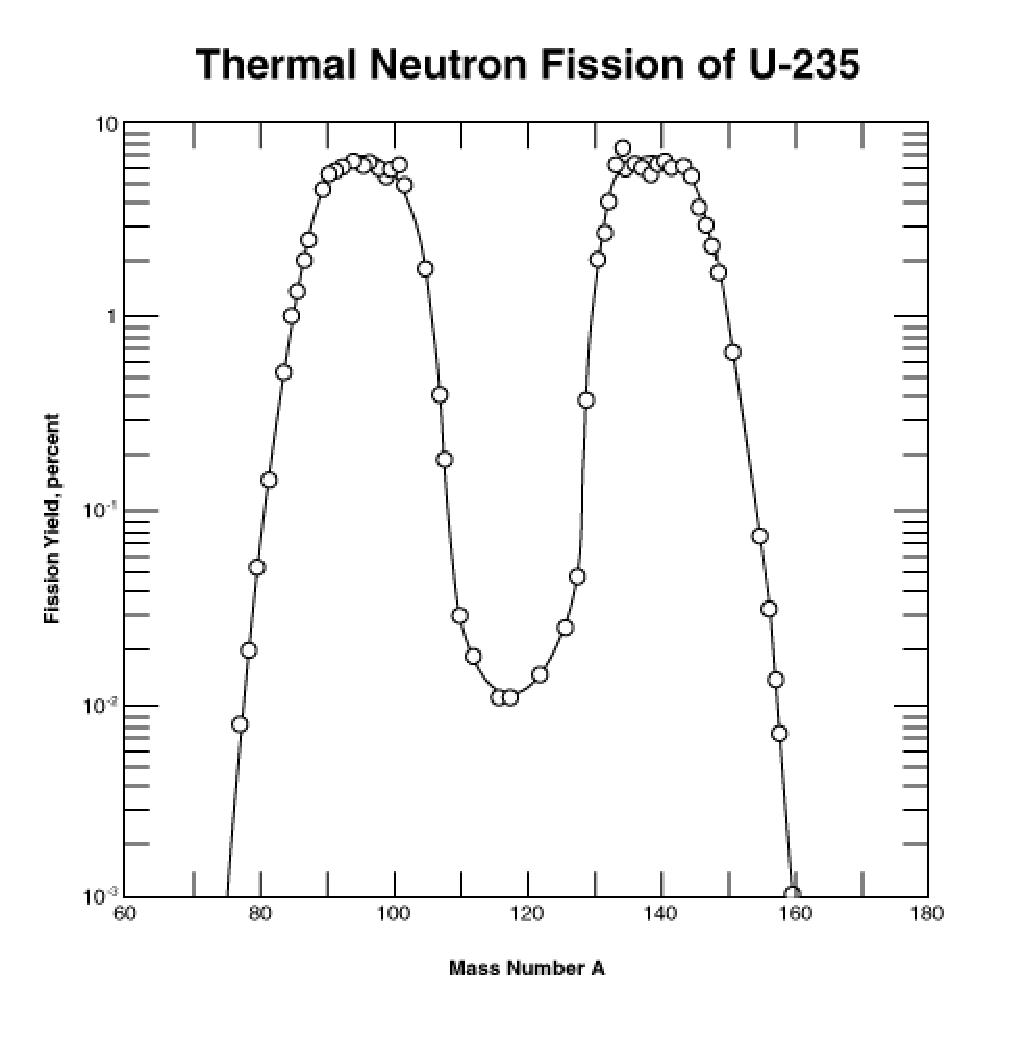
\includegraphics[scale=0.5]{figs/fissionyield}
	\end{center}
	\legend{Fonte: Physics of Uranium and Nuclear Energy\cite{14physics_uranium}, acesso em 07/05/2018 às 22:00}
\end{figure}

Notamos que existem dois picos de probabilidade, um em massas por
volta de 95u e outro em massas por volta de 150u, ou seja, normalmente
será formado um elemento mais leve e um elemento mais pesado, sendo
que é pouco provável que sejam formados elementos de massas similares.
Uma das reações possíveis de fissão do $^{235}U$ está descrita a
seguir:

\[
^{235}U+n\longrightarrow^{141}Ba+^{92}Kr+3n
\]

Como podemos ver, esta reação específica consome um nêutron lívre,
entretanto libera três nêutrons, ou seja, o saldo é positívo e é possível
sustentar a reação em cadeia. 

Tendo assegurada a capacidade de sustentar a reação em cadeia e utilizando
um arranjo de combustível favorável, surgem as necessidades associadas
às outras propriedades neutrônicas do reator, em especial neste trabalho
a reação de absorção seguida de captura será especialmente importante
pois é o princípio fundamental dos elementos férteis. As propriedades
neutrônicas se referem às formas como um nêutron pode interagir com
um dado material, em termos gerais, uma colisão pode resultar em uma
absorção ou espalhamento sendo que quando ocorre a absorção pode ocorrer
fissão ou captura. A propriedade que define a probabilidade de uma
dada interação ocorrer quando um nêutron colide com um núcleo é denominada
secção de choque e será tratada posteriormente neste trabalho.

\subsection*{Reatores de Óxido Misto}

Existe uma grande preocupação em relação ao processo de enriquecimento de Urânio, principalmente em discussões associadas ao uso militar da energia nuclear. A preocupação associada ao uso de combustíveis HEU (\emph{Highly Enriched Uranium} \textendash{} Urânio Altamente Enriquecido), ou seja, com enriquecimentos de mais de 20\% de $^{235}U$ é justificável e deve ser levada em consideração. Considerando que houvesse uma forma de reduzir a quantidade global de Urânio utilizado no reator sem alteração na produção de energia, esta solução seria muito bem vinda, principalmente aos olhos da comunidade internacional. 

Reatores de óxido misto são reatores nucleares capazes de queimar combustíveis compostos parcialmente de elementos chamados férteis, ou seja, que se tornam passiveis de fissão atômica quando ocorre a transmutação através da captura de um nêutron pelo átomo. O balanço entre elementos naturalmente físseis, como o $^{235}U$, e elementos férteis é calculado no combustível para que seja alcançada a criticidade e gerada energia com um consumo menor de Urânio. 

Dentre os elementos férteis, destaca-se no Brasil principalmente o Tório, devido às robustas reservas disponíveis, segundo dados da Agencia Internacional de Energia Atômica (IAEA), em 2005 as reservas de Tório no Brasil estavam estimadas em 606.000 mil toneladas, enquanto as reservas de Urânio estavam estimadas em 155.000 toneladas\cite{14physics_uranium}, se considerarmos que o Tório pode ser utilizado como combustível em reatores nucleares, é possível que o Brasil se mantenha autossuficiente em produção de combustível nuclear com facilidade, além disso, o período pelo qual a autossuficiencia se sustenta é aumentado drasticamente,
a confiabilidade associada a uma produção que não depende de flutuações no mercado externo é uma vantagem que não pode ser mensurada.

O uso de Tório e Plutônio como elementos férteis, na composição de combustíveis nucleares ja é considerado desde o início do desenvolvimento da área nuclear, entretanto a predominância do ciclo de apenas um uso em reatores PWR, visando a viabilidade econômica como maior fator diretor no desenvolvimento dos projetos afastou de discussão este tópico, existem diversas vantagens (em especial, no espectro ambiental) nos ciclos de Th-U, Pu-U e Th-Pu como é evidenciado por MOREIRA.

Uma das maiores vantagens da utilização de combustíveis de óxido misto Th-U é o fato de que a produção de elementos transplutônicos é de até três ordens de magnitude menor. Isto significa que ocorre uma menor produção de resíduos, que por sua vez significaria uma menor necessidade de incineração\cite{9moreira}.

O núcleo de $^{232}Th$, assim como o núcleo de $^{238}U$, não é físsil, entretanto quando ocorre a captura de um nêutron, o $^{232}Th$ se transmuta para $^{233}U$, que é um núcleo físsil, através de dois decaimentos do tipo $\beta$. As reações de transmutação do $^{232}Th$ e do $^{238}U$ podem ser vistas à seguir .

\[
^{238}U+n\xrightarrow{n\gamma}{}^{239}U\xrightarrow{\beta}{}^{239}Np\xrightarrow	{\beta}{}^{239}Pu
\]

\[
^{232}Th+n\xrightarrow{n\gamma}^{233}Th\xrightarrow{\beta}^{233}Pa\xrightarrow{\beta}^{233}U
\]

O núcleo de $^{232}Th$ é 6 unidades de massa mais léve do que o núcleo de $^{238}U$, por isso são necessárias mais capturas sucessivas para produzir actinídeos menores, como o Amerício ($^{241}Am$) e o Cúrio ($^{247}Cm$)., elementos que dificultam o processo de reciclagem do combustível nuclear. Concluímos então que o uso de Tório como parte do combustível é benéfico no que diz respeito a reduzir a produção de Plutônio, Amerício, Cúrio e outros acntinídeos. É possível verificar utilizando simulações, conforme observado por NIFENECKER, MEPLAN e DAVID, que as doses de radiação associadas à resíduos de combustíveis de reatores PWR à Urânio por GWh gerado são de até três ordens de grandeza maiores no curto prazo (t<100 anos) e de até 4 ordens de
grandeza no longo prazo (t>10.000 anos). Isto considerando o cenário de apenas um uso do combustível, se considerarmos um ciclo de combustível Th-U, devemos também considerar que a maioria dos isótopos que são fonte da dosagem de radiação são gerados no núcleo, e portanto são, em grande parte, consumidos durante o reprocessamento\cite{21NIFNECKER}.

Entretanto é necessário também entender que o consumo de nêutrons do reator será maior, observando de outra forma, haverão menos nêutrons disponíveis no reator ao longo do tempo e essa regeneração deve ser um fator determinante quando o combustível é dimensionado. Em seu livro, NIFENECKER, MEPLAN e DAVID descrevem este problema da seguinte forma: a reação de fissão do $^{232}Th$ exige primeiro a transmutação para $^{233}U$, que por sua vez exige a captura de um nêutron, além disso ainda é necessário computar um número de nêutrons que podem ser capturados após a criação do elemento físsil ($\alpha$), ou seja, cada elemento
físsil necessita de $1+\alpha$ nêutrons e a criação de um novo elemento físsil necessita de outros $1+\alpha$ nêutrons, ou seja, para produção de uma fissão, são necessários $2(1+\alpha)$ nêutrons. Adicionado a isso ainda existe a prossibilidade de fuga ($L$ ), de forma que o fator de multiplicação $k$ é uma função do número de nêutrons médio disponível por fissão ($v$) e será dado por:

\begin{equation}
k=\frac{v}{2(1+\alpha)+L+N_{a}},
\end{equation}

onde:

\begin{equation}
\alpha=\frac{\sigma_{c}}{\sigma_{f}};
\end{equation}

$\sigma_{c}$ é a secção de choque de captura, $\sigma_{f}$ é a secção de choque de fissão e $N_{a}$ é o número médio de nêutrons gerados por fissão\cite[pag.~217]{21NIFNECKER}, observando este modelo simplificado, verifica-se que o fator de multiplicação depende da probabilidade de fuga, e da relação entre as probabilidades de captura e fissão do elemento. Lembrando também que estas energias variam se estivermos trabalhando no espectro térmico ou no espectro rápido.

\section{Dados Nucleares}

Os dados nucleares descrevem as relações que os nêutrons tem com os elementos presentes nos núcleos, de forma a determinar quais tipos de reações nucleares ocorrerão, a frequência de ocorrência e, além disso, o resultado das interações. Estas informações são de suma importância no dimensionamento de reatores e dos seus combustíveis, além de serem utilizadas em previsões e, obviamente, simulações. No centro do espectro de importância dos dados nucleares estão as informações de secção de choque, em termos mais simples, a área-alvo de um determinado nuclídeo em relação à um nêutron incidente. Este número não é apenas um dado
dimensional, é uma aproximação matemática. A secção de choque depende, dentre outros fatores, da energia cinética do nêutron.

Conforme pode ser observado em SHULTIS e FAW a secção de choque macroscópica é definida como sendo o produto da secção de choque microscópica pela densidade numérica de nucleos em um determinado meio, outra forma de observar é imaginando a mecânica probabilística, onde a secção de choque macroscópica é o inverso do caminho livre médio\cite{10fundamentos}.

\begin{equation}
\Sigma=N\sigma,
\end{equation}

\begin{equation}
\lambda=\frac{1}{\Sigma}.
\end{equation}

\subsection{Densidades numéricas}

A densidade numérica, juntamente com as secções de choque, é um dos fatores mais importantes na simulação de reatores nucleares. Seu calculo é feito através da densidade teórica ou experimental de um material ($\rho$), das massas molares ($A$) de cada um dos componentes desse material, da constante de avogadro ($N_{0}$) segundo a seguinte relação:

\begin{equation}
N=\frac{\rho N_{0}}{A},
\end{equation}

Ou seja:

\begin{equation}
\Sigma=\frac{\rho N_{0}\sigma}{A},
\end{equation}

É importante frisar que, em compostos multiatômicos, como é o caso da maioria esmagadora dos combustíveis nucleares, a densidade atômica é calculada considerando todos os átomos da molécula.

\subsection{Faixas de energia de nêutrons}

Como ja foi citado, outro fator importante para a definição das secções de choque é a faixa de energia cinética do nêutron incidente, definimos as secções de choque macroscópica como funções de $E$, ou seja $\sigma\rightarrow\sigma(E)$ e $\Sigma\rightarrow\Sigma(E)$. Conforme observado também em SHULTIS E FAW, experimentalmente existem três faixas de energia com as quais os nêutrons podem ser produzidos após uma fissão\cite{10fundamentos}:
\begin{itemize}
\item Energias altas, que variam de 0,1 MeV até 10 MeV (nêutrons rápidos), nessa faixa a energia é alta o suficiente para que as propriedadesvibracioais do meio não interfiram substancialmente no espalhamento dos nêutrons, a taxa de reação causada por estes nêutrons é alta devido às suas altas velocidades.
\item Energias baixas, que variam de 0,001eV até 1,0 eV (ou nêutrons térmicos), nessa faixa, a energia é baixa, de forma que a vibração dos átomos que compõe o meio de propagação interfere no espalhamento dos nêutrons, para reatores PWR estes nêutrons são especialmente importantes pois suas velocidades baixas permitem que o sistema tenha constantes de tempo de faixas mais controláveis. 
\item Energias intermediárias, que vão de 1,0 eV até 1,0 MeV.
\end{itemize}
A distribuição de número de átomos gerados em fissões em relação à energia cinética dos mesmos pode ser observada no gráfico a seguir:

\begin{figure}[htpb]
	\caption{\label{PWR} Secção de choque dos nêutrons gerados na fissão do U-235 em relação à sua energia.}
	\begin{center}
	    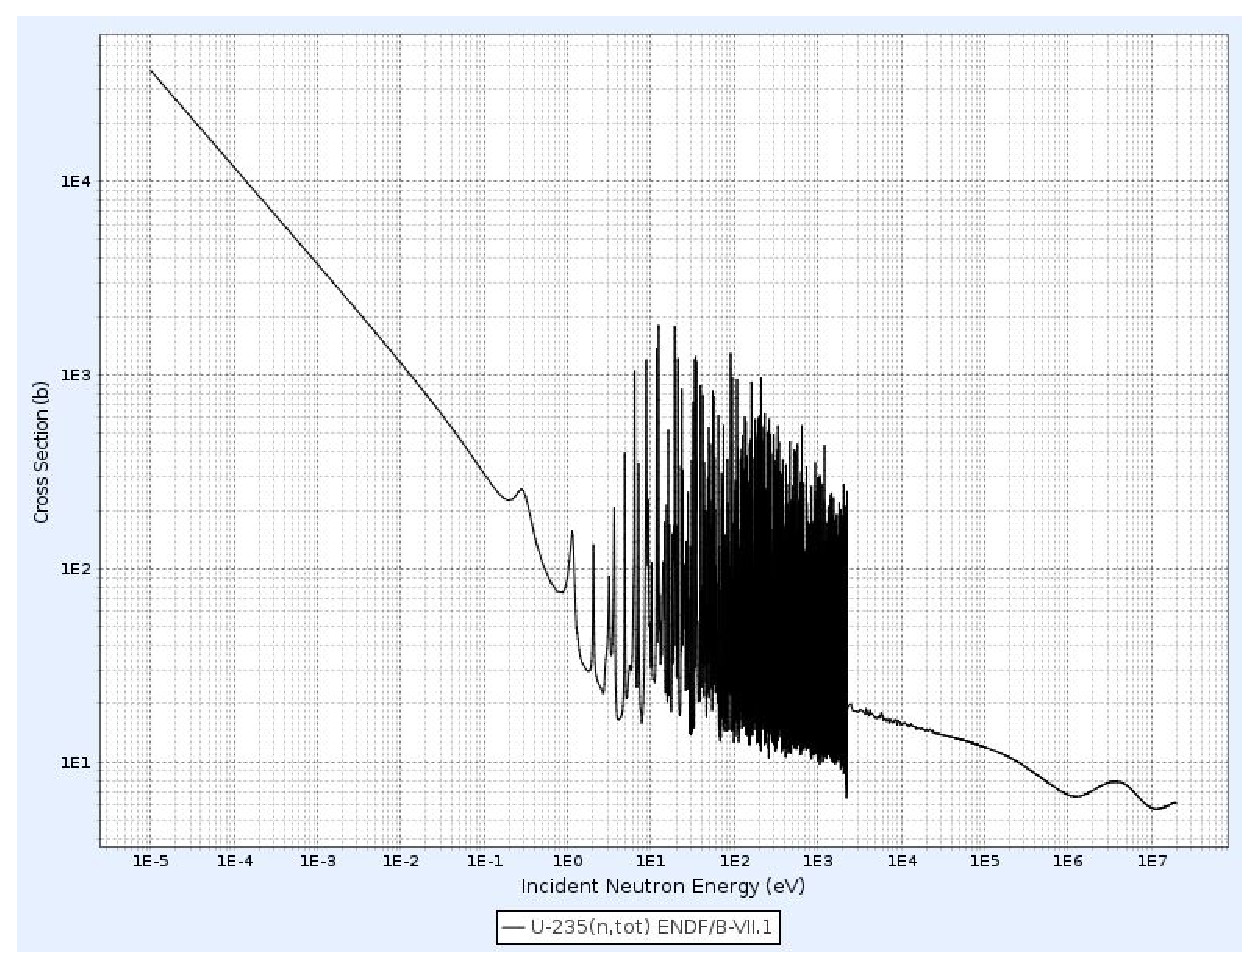
\includegraphics[scale=0.5]{figs/secao_de_choqueXenergiaU235}
	\end{center}
	\legend{Fonte: http://atom.kaeri.re.kr/nuchart/, acesso em 07/05/2018 às 21:30}
\end{figure}

\section{O método Monte Carlo}

Dentre os métodos utilizados para simulações na atualidade, o que mais se destaca é, sem dúvida, o método de Monte Carlo. O método consiste de um modelo estocástico construído de forma que o valor esperado de uma determinada variável aleatória seja equivalente a uma certa quantidade física a ser determinada. Tal valor esperado é determinado por uma gama de amostras independentes selecionadas por intermédio de uma variável aleatória obtida por intermédio de números pseudoaleatórios
associados a uma distribuição específica que representa o fenômeno em questão\cite{4montecarloprinciples} \cite{5pedrao}. No método de Monte Carlo devemos seguir a partícula desde seu nascimento (a fonte) ate sua morte (absorção ou escape). A distribuição de probabilidades é amostrada aleatoriamente usando os dados nucleares de transporte\cite{6nextgeneration} para determinar o resultado da interação cada a etapa de vida da partícula. Técnicas específicas devem ser implementadas para problemas críticos, onde o comprimento da cadeia de nêutrons pode alcançar o infinito. Dentre os códigos recentemente desenvolvidos para a simulação da física de reatores se encontra o código MCNP\cite{8MCNP}, que é um sistema de simulação de física de reatores via método de Monte Carlo desenvolvido pelo LANL.

A aplicação do código se da através do software MCNPX. A mecânica é feita por amostragem pseudorrandômica, onde são gerados parâmetros aleatórios a partir de uma situação inicial. Para que seja realizada a simulação, são realizados os seguintes questionamentos para cada ciclo de simulação dada um estado inicial: 
\begin{itemize}
\item Se o nêutron reage com o meio; 
\item Caso haja reação, com quais nuclídeos; 
\item Caso haja reação, quais tipos de reação são possíveis; 
\item Para cada reação ocorrida, quais partículas são emitidas.
\end{itemize}
A probabilidade de reação ou não do nêutron com o meio está relacionada
a sua secção de choque macroscópica da partícula no meio tratado ($\Sigma_{t}$).
De forma geral, a partir de um ponto inicial $l$, dado um diferencial
qualquer de distância $dl$ percorrido em um determinado meio, a probabilidade
do nêutron sofrer uma colisão é de:

\begin{equation}
p(l)dl=\exp(-\Sigma_{t}l)\Sigma_{t}dl
\end{equation}

A partir desta relação, considerando um número aleatório $\xi$ distribuído
no intervalo $(0,1]$, integrando a equação $(1),$ teremos:

\begin{equation}
\xi=\intop_{0}^{1}p(l')dl'=1-\exp(-\Sigma_{t}l)
\end{equation}

Onde pode ser concluído que $l$ é a distância mínima até a posição da colisão mais próxima. Dada a posição inicial da partícula, através dos parâmetros fornecidos utilizando uma amostragem específica, pode ser calculada a distância até a fronteira da célula mais próxima. Se a distância $l$ é maior do que a distância entre a partícula e a fronteira mais próxima, então a partícula é movida para a fronteira, caso contrário considera-se que a colisão ocorre na posição $l$. Existem dois tratamentos possíveis para os nêutrons gerados em reações nucleares, o tratamento dado é definido a partir da energia do nêutron. Em condições de baixa energia (nos denominados nêutrons lentos) e em casos como a água ou o grafite, os efeitos de rede cristalina se tornam
mais importantes e estes efeitos são adicionados à equação através das funções de transferência $S(\alpha,\beta)$, onde $\alpha$ é o momento transferido e $\beta$ a energia transferida corrigida. As funções de transferência são tabeladas e disponíveis em bibliotecas de arquivos ENDFB. Em casos de alta energia, ou em modelos onde o meio é um gás livre o tratamento é o mesmo, considera-se que a secção de choque à temperatura zero é independente da temperatura do nêutron incidente e a secção de choque da reação independente da temperatura do meio.

\begin{equation}
\sigma(T)=\sigma(0)(1+\frac{kTAEn}{2})
\end{equation}

Onde A é o peso atômico do sítio de colisão e En é a energia do nêutron ( a expressão utilizada é válida enquanto $\sqrt{\frac{AEn}{kT}}>2$, em outros casos é utilizado uma relação mais geral). A colisão é modelada considerando o alvo como estacionário, sendo que a velocidade do nêutron em relação ao alvo é determinada através da distribuição de Maxwell.

O nuclídeo com o qual ocorre a reação é determinado através da secção de choque macroscópica, de forma que é sabido que a somatória da probabilidade de reação de todos os nuclídeos que compõe o meio é igual a 1, sendo assim é gerado um número aleatório $\eta\epsilon(0,1]$. As probabilidades de cada um dos nuclídeos são somadas em uma determinada ordem, o nuclídeo
$n$ será selecionado se $\eta$ estiver contido no intervalo demarcado pela probabilidade deste nuclídeo. A reação que ocorre após a colisão é determinada através da secção de choque microscópica de cada uma das reações segundo a biblioteca do programa, onde a probabilidade de uma reação $i$ ocorrer depende da secção de choque total de reação ($\sigma_{t})$ e é dada por; $P(i)=\frac{\sigma_{i}}{\sigma_{t}}$. A mecânica da simulação que seleciona qual reação ocorre é exatamente a mesma mecânica que seleciona com qual nuclídeo o nêutron colidirá, a mudança é que consideramos as probabilidades associadas a cada uma das secções de choque dos nuclídeos, sendo que a somatória de todas as secções de choque microscópicas é a secção de choque microscópica
total.
As partículas produto das reações nucleares são lançadas com direções e energias definidas aleatoriamente, em termos gerais, considera-se que a probabilidade de espalhamento em todas as direções é dada por:

\begin{equation}
\intop_{0}^{^{2\pi}}\intop_{0}^{\pi}P(\delta,\theta)d\delta d\theta=1
\end{equation}

O processo que decide em qual direção ocorrerá o espalhamento se da de forma mais complexa, porém, similar a seleção do nuclídeo com o qual o nêutron interage, as probabilidades relacionadas a cada ângulo são determinadas através das tabelas de distribuições angulares, presentes nas bibliotecas do programa. Após finalizada a reação nuclear, é retomado o processo iterativo a partir do passo de determinação de $l$. O método realiza o cálculo para quantos ciclos de reação são determinados no parâmetro fonte de fissão (kcode). 

\subsection{O código MCNP}

O programa lê um arquivo denominado input, selecionado antes do inicio da simulação, o código deve ser estruturado sempre da mesma forma, sendo que o mesmo é dividido em três segmentos, denominados cartões\cite{8MCNP}.
\begin{itemize}
\item Cartões de Superfície: Definem espaços geométricos que posteriormente serão utilizados para conformar as células. 
\item Cartões de Célula: Os componentes do reator simulado (barras de combustível, moderador etc) são definidos através dos cartões de célula, cada célula é definida a partir do vetor diretor de um ou mais espaços definidos pelos cartões de superfície. 
\item Cartões de Dados: Existem três tipos de Cartões de Dados, os do cartões do tipo fonte (ksrc), os cartões do tipo código (kcode) e os cartões de materiais. Os cartões do tipo fonte definem os nêutrons que existem no reator no inicio da simulação, os cartões do tipo código especificam como o programa fará a simulação, já os cartões de materiais especificam a biblioteca da qual serão obtidas as informações dos materiais, além da composição específica de cada um dos materiais em caso de ligas metálicas.
\end{itemize}

\subsubsection*{Cartões de superfície }

Os Cartões de Superfície são representados por um número identificador
único, um mnemônico tabelado e uma série de parâmetros que diferem
quantitativamente e qualitativamente para cada mnemônico, a tabela
completa dos mnemônicos se encontra a seguir.

\newpage
\begin{center}
\begin{longtable}{|l|l|l|}
\caption[Mnemônicos dos cartões de superfície do código MCNP]{Mnemônicos dos cartões de superfície do código MCNP}

\label{SUPMNEMONICS} \\

% header ------------------------
\hline

Mnemônico & Equação & Entradas\tabularnewline
\hline 
\hline 
P & $Ax+By+Cz-D=0$ & $A,B,C,D$\tabularnewline
\hline 
PX & $x-D=0$ & $D$\tabularnewline
\hline 
PY & $y-D=0$ & $D$\tabularnewline
\hline 
PZ & $z-D=0$ & $D$\tabularnewline
\hline 
SO & $x^{2}+y^{2}+z^{2}-R^{2}=0$ & $R$\tabularnewline
\hline 
S & $(x-\bar{x})^{2}+(y-\bar{y})^{2}+(z-\bar{z})^{2}-R^{2}=0$ & $x,y,z,R$\tabularnewline
\hline 
SX & $(x-\bar{x})^{2}+y^{2}+z^{2}-R^{2}=0$ & $x,R$\tabularnewline
\hline 
SY & $x^{2}+(y-\bar{y})^{2}+z^{2}-R^{2}=0$ & $y,R$\tabularnewline
\hline 
SZ & $x^{2}+y^{2}+(z-\bar{z})^{2}-R^{2}=0$ & $z,R$\tabularnewline
\hline 
C/X & $(y-\bar{y})^{2}+(z-\bar{z})^{2}-R^{2}=0$ & $y,z,R$\tabularnewline
\hline 
C/Y & $(x-\bar{x})^{2}+(z-\bar{z})^{2}-R^{2}=0$ & $x,z,R$\tabularnewline
\hline 
C/Z & $(x-\bar{x})^{2}+(y-\bar{y})^{2}-R^{2}=0$ & $x,y,R$\tabularnewline
\hline 
CX & $y^{2}+z^{2}-R^{2}=0$ & R\tabularnewline
\hline 
CY & $x^{2}+z^{2}-R^{2}=0$ & R\tabularnewline
\hline 
CZ & $x^{2}+y^{2}-R^{2}=0$ & R\tabularnewline
\hline 
K/X & $\sqrt{(y-\bar{y})^{2}+(x-\bar{x})^{2}}-t(x-\bar{x})=0$ & $x,y,z,t^{2}\pm1$\tabularnewline
\hline 
K/Y & $\sqrt{(x-\bar{x})^{2}+(z-\bar{z})^{2}}-t(y-\bar{y})=0$ & $x,y,z,t^{2}\pm1$\tabularnewline
\hline 
K/Z & $\sqrt{(y-\bar{y})^{2}+(x-\bar{x})^{2}}-t(z-\bar{z})=0$ & $x,y,z,t^{2}\pm1$\tabularnewline
\hline 
KX & $\sqrt{y^{2}+z^{2}}-t(x-\bar{x})=0$ & $x,t^{2}\pm1$\tabularnewline
\hline 
KY & $\sqrt{x^{2}+z^{2}}-t(y-\bar{y})=0$ & $y,t^{2}\pm1$\tabularnewline
\hline

\end{longtable}
\legend {Fonte: MCNP Manual}
\end{center}


Os elementos gerados através do cartão de superfície são os espaços matemáticos representados por suas funções, cada cartão de superfícierepresenta uma figura num espaço a partir de um referencial e estas figuras simples são utilizadas para construir figuras mais complexas. Cada superfície representa uma superfície de algum componente do alvo da simulação (no caso, de um reator), sendo que uma mesma superfície pode ser utilizada como base para dois ou mais Cartões de Célula (no caso de intersecções) como será explicado na etapa seguinte. A forma que utilizamos para combinar os cartões de superfície em figuras
complexas são os cartões de célula.

\subsubsection*{Cartões de célula }

Um cartão de célula é composto por cinco partes principais: um número identificador geral, um número identificador de material
(que é relacionado com o cartão de material), um identificador de densidade que pode ser atômica ou mássica, os parâmetros que definem os limites da célula e o parâmetro imp:n.

\begin{itemize}
\item Identificador de Material: É um número natural compartilhado com o
material do qual é composta a célula descrita;
\item Identificador de Densidade: É um número real que, se positivo, indica
a densidade atômica do material que compõe a célula descrita e, se
negativo, indica a densidade mássica do material.
\item Parametros de Limite de Célula: São um conjunto de números inteiros
que definem o limite da célula através de relações que são equivalentes
às de um Diagraa de Venn tridimensional, cada número se associa a
um cartão de superfície e o sinal associado ao número indica se a
zona tratada está a favor ou contra o vetor diretor da superfície
identificada pelo número.
\item Parâmetro imp:n: É um número binário que define se a célula criada
faz parte ou não dos limites da simulação, ou seja, se os nêutrons
que por ventura cruzarem o limite da célula devem ser simulados posteriormente
ou se devem ser considerados perdidos, sendo que quando o parâmetro
é regulado em 0 a célula é considerada fora dos limites da simulação
e quando o parâmetro é regulado em 1 a célula é considerada dentro
dos limites da simulação. 
\end{itemize}
Os mnemônicos utilizados neste trabalho para relacionar os cartões
de superfície e gerar os cartões de célula estão descritos na tabela
a seguir:

\begin{center}
\begin{longtable}{|l|l|l|}
\caption[Mnemônicos mais relevantes para os cartões de célula do código MCNP]{Mnemônicos mais relevantes para os cartões de célula do código MCNP}

\label{CELLMNEMONICS} \\

% header ------------------------
\hline
Mnemônico & Significado\tabularnewline
\hline 
\hline 
Espaço simples & União de duas superfícies\tabularnewline
\hline 
: & Intersecção de cartões de superfície\tabularnewline
\hline 
u=n & Cria um objeto que pode ser copiado e manipulado ($n\in N$)\tabularnewline
\hline 

\end{longtable}
\legend {Fonte: MCNP Manual}
\end{center}
A principal ferramenta do software utilizada neste trabalho para modelar o reator nuclear é a ferramenta latt, que é utilizada para repetir estruturas com alteração da referência central, utiliza-se esta ferramenta para modelar os conjuntos de barras de controle, de tubos-guia e de varetas de combustível.

\subsubsection*{Cartões de materiais}

Os cartões de materiais especificam, como o proprio nome implica, os materiais dos quais são feitas as diferentes células apresentadas nos cartões de células, o código do cartão de material vinculado a um material específico é composto de três partes importantes: o identificador sequencial atrelado à letra m, o identificador do componente que é composto pelo número atômico associado ao número de massa e à biblioteca do MCNPX, da qual serão extraídas as informações de secção de choque
e finalmente a fração normal do composto observado. Não há limites para complexidade na composição de um determinado material, sendo que a regra é sempre que o identificador é apresentado antes da fração normal para cada um dos componentes. A estrutura de um cartão de material simples, para plutônio natural pode ser observada a seguir:

\begin{lstlisting}
C Materials Cards  
m1   94239.66c 3.7047e-2 
     94240.66c 1.751e-3  
     94241.66c 1.17e-4 
     31000.66c 1.375e-3
\end{lstlisting}

Há também a possibilidade de considerar as alterações na secção de
choque dos elementos quando ocorrem interações específicas, por exemplo
quando os mesmos estão em contato com água, através da utilização
do comando lwtr.01t, que é aplicado ao cartão de materiais com o mesmo
numero natural utilizado após o ponto no comando.

\subsubsection*{Cartões de Controle}

O Método Monte Carlo se fundamenta na geração de números aleatórios
baseados em uma condição inicial dado um número de ciclos de iteração,
no código MNCP este conjunto de parâmetros é fornecido através dos
cartões de controle.

O trecho kcode do cartão de controle especifica parâmetros de ensaio,
como por exemplo após quantos ciclos de simulação será iniciada a
coleta de dados e por quantos ciclos de simulação será feita a coleta
após o início, isto se torna especialmente importante quando temos
ensaios onde é necessário estudar condições desenvolvidas como gasto
de combutível ou criticidade, estas condições não são observáveis
quando a simulação está em seus instantes iniciais. São 4 algarismos
equenciais, o primeiro (nsrck) define o número de nêutrons que serão
simulados por ciclo de simulação, o segundo (rkk) define o $k_{ef}$
do instante inicial da simulação, o terceiro (ikz) define o número
de ciclos de simulação antes do inicio da aquisição de dados e o quarto
(kct) define o número de ciclos de simulação que serão conduzidos.

O trecho ksrc define as condições iniciais dos nêutrons dentro do reator, no instante t=0 a distribuição de nêutrons é exatamente a explicitada neste trecho. Existem muitas opções para a seleção da condição inicial ideal para cada simulação, o programa apresenta opções que vão desde nêutrons pontuais com três coordenadas de posição inicial até distribuições heterogêneas que seguem padrões equacionados (como é o caso da fonte utilizada no experimento deste trabalho). Para n
nêutrons são dadas as três coordenadas iniciais em sequência separadas por um espaço nêutron: $x_{n1}$ $y_{n1}$ $z_{n1}$ $x_{n2}$ $y_{n2}$ $z_{n2}$ ... $x_{nn}$ $y_{nn}$ $z_{nn}$.

O cartão de controle a seguir preve um ponto de partida com um nêutron
na origem, são simulados 5000 nêutrons por iteração do código com
$k_{ef}$ inicial de 1,0. Serão realizados 50 ciclos antes do início
da coleta de dados, que por sua vez será feita durante 250 ciclos.

\begin{lstlisting}
C Criticality Control Cards  
kcode 5000 1.0 50 250  
ksrc 0 0 0
\end{lstlisting}

\newpage
\section{Justificativa}

Na intenção de viabilizar futuros experimentos relacionados a o uso de ciclos de combustíveis Th-U, é necessário descobrir se os dados nucleares básicos do nuclídeo tório estão suficientemente satisfatórios do ponto de vista de projeto de reatores nucleares.

O projeto busca responder esta pergunta através da proposição de um arranjo crítico de um núcleo contendo óxido de tório para o reator IPEN/MB-01. Tal núcleo pode servir de base para futuras comparações intencionadas a verificar e validar os dados nucleares básicos do tório.



% ---
% Capitulo Sobre a Modelagem
% ---
\chapter{Modelagem e Aproximações}
% ---

\section{O Reator IPEN/MB-01}

O reator nuclear IPEN/MB-01\cite{1reator} consiste de um reator nuclear dedicado
a pesquisa básica e aplicada em física de reatores e áreas correlatas,
sua potência nominal é limitada a 100 Watts e por isso é chamado de
um reator de potência \textquotedblleft zero\textquotedblright . O
sistema nuclear é constituído por um núcleo contendo material físsil
distribuído em um arranjo regular de forma a possibilitar a manutenção
da reação em cadeia. Sua principal aplicação é a comprovação das metodologias
utilizadas para a área de física de reatores para projetos e experimentos.
Construtivamente, seu primeiro e atual núcleo, está contido em um
barril de aço inoxidável, e em sua forma padrão é composto por 680
varetas de elementos combustível, cada uma das quais constituídas
de pastilhas de dióxido de Urânio enriquecido a 4,3 \% em Urânio 235
somados a 48 barras absorvedoras responsáveis pelo controle e segurança
do reator. O objetivo principal da instalação prima pela avaliação
em escala real de parâmetros nucleares, e atualmente é considerada
padrão de referência internacional via participação em \textquotedblleft benchmarks\textquotedblright \cite{2handbook}\cite{3international} internacionais dedicados ao tema.

\subsection{Tanque Moderador}

O tanque moderador do MB-01 é, como ja foi mencionado, um cilindro
de aço inoxidável que possui uma abertura superior, sua medida de
dâmetro externo é de 1830mm, sua largura é de 2750mm e o mesmo é feito
de aço com 8,5mm de expessura, o aço inoxidável utilizado é o ASTM
SS-304. Como padrão de operação, o nível de água permanece sempre
450mm acima da região ativa do núcleo, onde ocorre a queima de combustível.

A distância da região ativa do núcleo para as bordas do cilindro de aço é de, no ponto mínimo, 600mm e a profundidade de água abaixo da região ativa é de 530mm. 

\subsection{Núcleo do Reator}

O nucleo do reator é composto por um arranjo de até 30 por 30 varetas identicas dimensionalmente, mas é mais comumente utilizado no arranjo 26x28, alocadas em uma matriz (composta de três placas perfuradas),resultando no formato de um paralelepípedo de dimensões 390mm por 420mm por 546mm, estas varetas são divididas em:
\begin{itemize}
\item 24 Barras de Controle
\item 24 Barras de Segurança
\item 680 Varetas de Combustível
\end{itemize}
A figura~\ref{sidecore} apresenta o arranjo contendo o tanque moderador e o núcleo do reator em visão lateral, o experimento conduzido considerou este arranjo padrão para as varetas, os ajustes foram feitos apenas na composição da parte ativa das mesmas.

\begin{figure}[htpb]
	\caption{\label{sidecore}Diagrama de visão lateral do nucleo do reator MB-01.}
	\begin{center}
	    \includegraphics[scale=1]{figs/Core_Side}
	\end{center}
	\legend{Fonte: CRITICAL LOADING CONFIGURATIONS OF THE IPEN/MB-01 REACTOR WITH HEAVY REFLECTORS COMPOSED OF CARBON STEEL AND NICKEL\cite{20figuras}}
\end{figure}

Na visão superior apresentada na figura~\ref{topreactor} podemos ver a localização
de cada um dos 728 cilindros, as barras de controle, apresentando
a letra C, são utilizadas para controle da criticidade do reator a
curto prazo, usualmente são operadas por um sistema de controle avançado,
as barras apresentando a letra S são utilizadas em caso de emergência,
onde a criticidade do reator precisa se reduzida com grande velocidade
para evitar vazamentos ou outros problemas, este sistema é operado
por outro controle avançado mas pode ser acionado pela operação do
reator em caso de falha do controle. O ajuste fino na criticidade
do reator é feito através da dosagem de um sal de Boro na água que
modera o sistema, minimizando a atuação das barras de controle.

\begin{figure}[htpb]
	\caption{\label{topreactor}Diagrama de visão superior do reator MB-01 com detalhe.}
	\begin{center}
	    \includegraphics[scale=1]{figs/Reactor_TOP_VIEW}
	\end{center}
	\legend{Fonte: CRITICAL LOADING CONFIGURATIONS OF THE IPEN/MB-01 REACTOR WITH HEAVY REFLECTORS COMPOSED OF CARBON STEEL AND NICKEL\cite{20figuras}}
\end{figure}
\newpage

\subsection{Matrizes de Furos}

A matriz onde são alocadas as varetas e as barras de controle (para garantia de alinhamento correto) é composta de três placas de aço perfuradas, a placa superior tem espessura de 20mm com furos passantes para todas as barras de controle e varetas combustíveis, a placa intermediária fica a 210mm da base da placa superior e tem 10,5mm, os furos tem a mesma distribuição da placa superior, a placa inferior fica a 890mm da base da placa intermediária e não possui furos passantes, apenas cavidades de 12mm de profundidade onde se alojam as pontas de todas as varetas e barras, a placa inferior tem 22mm de expessura. 

A figura~\ref{matrix} apresenta o arranjo das placas da matriz conforme apresentado,
assim como a incerteza para cada uma das grandezas.

\begin{figure}[htpb]
	\caption{\label{matrix}Diagrama de visão lateral do nucleo do reator MB-01 com detalhe para as matrizes de furos.}
	\begin{center}
	    \includegraphics[scale=0.75]{figs/Matrix_SIDE_VIEW}
	\end{center}
	\legend{Fonte: CRITICAL LOADING CONFIGURATIONS OF THE IPEN/MB-01 REACTOR WITH HEAVY REFLECTORS COMPOSED OF CARBON STEEL AND NICKEL\cite{20figuras}}
\end{figure}

\subsection{Varetas de Combutível}

As varetas de combustível padrão do reator são tubos de aço inox AISI-304 que contem 54 pastilhas de Óxido de Urânio enriquecido em seu interior, cada pastilha tem altura de 10,5mm e 8,49mm de diâmetro. As extremidades inferior e superior das varetas não são ativas e são preenchidas com pastilhas de Alumina com as mesmas dimensões das pastilhas de Óxido de Urânio, a figura~\ref{vareta} apresenta o diagrama de uma vareta. Na extremidade inferior das varetas há um cone cortado, que possui encaixe na matriz inferior, para fixação da vareta.
\begin{figure}[htpb]
	\caption{\label{vareta}Diagrama de visão lateral de uma vareta combustível do MB-01.}
	\begin{center}
	    \includegraphics[scale=1]{figs/VARETA_SIDE_VIEW}
	\end{center}
	\legend{Fonte: CRITICAL LOADING CONFIGURATIONS OF THE IPEN/MB-01 REACTOR WITH HEAVY REFLECTORS COMPOSED OF CARBON STEEL AND NICKEL\cite{20figuras}}
\end{figure}

\newpage
\subsection{Barras de Controle e Segurança}

As barras utilizadas para redução de criticidade são movimentadas
sempre em grupos de 12, ou seja, são dois bancos de barras de controle
e dois bancos de barras de segurança, todas as 48 barras são dimensionalmente
identicas e revestidas também de aço ASTM SS-304 sendo que as barras
de controle são recheadas com uma liga de Ag-In-Cd e as barras de
segurança são recheadas com Carbeto de Boro ($B_{4}C$), um composto
que é forte absorvedor de nêutrons.

Usualmente a grandeza que determina quanto de cada um dos bancos de controle está inserido no reator é calculada com relação ao comprimento total da barra em relação ao comprimento que ultrapassou o limite definido pela matriz de furos superior, mais especificamente o quanto das barras de controle não está inserido no nucleo, a grandeza é denominada percentagem retirada. Para configurações que visam economia de combustível é ideal trabalhar com valores de percentagem retirada próximos à 100\%, pois a inserção das barras de controle absorvem nêutrons que de outro modo estariam desencadeando novas reações e gerando energia, este
ajuste fino é feito através do ajuste da composição das varetas ao longo da matriz do núcleo, de forma a posicionar varetas com maior concentração de $^{235}U$ (ou seja, mais novas) nas camadas exteriores e varetas com menor concentração de $^{235}U$ nas camadas interiores. A figura~\ref{fotocore} apresenta uma foto do núcleo do reator onde podem ser vistas as 4 hastes que controlam os 4 bancos de controle e de segurança completamente inseridas (pois o vaso de contenção do reator está aberto), ou seja com percentagem de retirada de 0\%.

\begin{figure}[htpb]
	\caption{\label{fotocore} Foto do núcleo do MB-01 durante uma parada da unidade.}
	\begin{center}
	    \includegraphics[scale=1]{figs/FOTO_NUCLEO}
	\end{center}
	\legend{Fonte: https://www.ipen.br/, acesso em 07/05/2018 às 20:00.}
\end{figure}

\part*{Características da Modelagem Utilizada}

Os ensaios sugeridos por MOREIRA, em 1998, atendem até certo ponto a necessidade apresentada na introdução deste trabalho, entretando, em virtude de uma ótica diferente e usufruindo da versatilidade oferecida pelo método computacional, o estudo no reator MB-01 foi realizado de forma diferente da sugerida. Para todos os arranjos e proporções Tório-Urânio a simulação foi realizada utilizando os mesmos parâmetros iniciais e durante o mesmo número de cíclos. As composições utilizadas 
para o combustível nas varetas foram as mesmas propostas por MOREIRA em seu trabalho.

\section{Varetas de Ensaio}

As varetas de ensaio apresentadas por MOREIRA foram desenvolvidas
para minimizar os efeitos de borda sobre o elemento estudado, ou seja,
o Thório está presente apenas na região central das varetas, sendo
que as pastilhas contendo as composições de Thório estão entre camadas
de pastilhas de Urânio. Uma vareta de ensaio proposta por MOREIRA
contém pastilhas de Óxido de Thório e pastilhas de Óxido de Urânio,
sendo que o invólucro das pastilhas é sempre o mesmo, as varetas de
ensaio não são distinguiveis visivelmente das varetas de combustível
comuns do reator.

Entretanto, tendo em vista que este trabalho visa apresentar uma proposta
de ensaio real, contemplando também a dificuldade adiconal de manufaturar
as varetas corretamente utilizando o projeto proposto por MOREIRA,
foram utilizadas varetas com recheio de Tório puro, descartando as
regiões com Urânio enriquecido que ficariam acima e abaixo da região
do Tório. Uma das preocupações de MOREIRA era com a redução na reatividade
induzida pelo Tório, que poderia não permitir a sustentação da reação
em cadeira, os resultados permitiram observar que este arranjo é possível
e resulta em valores de k acima de 1.

Para modelagem das varetas utilizou-se um novo objeto (no programa,
chama-se universo), através do mnemônico ``u'', com as mesmas caracteríticas
dimensionais de uma vareta comum, adicionando apenas o cilindro central
contendo as frações, descritas na proxima seção do trabalho, de Óxido
de Thório, o código utilizado é o seguinte:

\begin{lstlisting}
c  Thorium Rod  
c ccccccccccccccccccccccccccccccccccccc 
c 
c  Thorium pellets 
c 
101  14   6.9450e-02         
          (-1 3 -2)
          imp:n=1
          u=9 
c 
c  aluminum stopple up 
c 
102  5    1.118600e-01
          (-5 2 -4)
          imp:n=1
          u=9 
c 
c  aluminum stopple botton 
c 
103  5    1.118600e-01
          (-5 -3)
          imp:n=1
          u=9 
c 
c Spacer Tube 
c  
104  7    8.802220E-02
          (4 -7 6)
          imp:n=1
          u=9
c 
c Gap  
c 
105  2    -1.20492E-3
          (5 -7  2 -4 ):   $ gap top
          (5 -7 -3    ):   $ gap botton
          (3 -2  1 -7 ):   $ gap U02
          (7 -9       )    $ gap
          imp:n=1
          u=9 
c 
c Void 
c 
106    0
       (-6 4)
       imp:n=1
       u=9 
c 
c Cladding 
c 
107  3    8.655893e-02
          (9 -10)
          imp:n=1
          u=9 
c 
c Water  
c  
108  4    1.00104E-01
          (10)
          imp:n=1
          u=9
\end{lstlisting}

Temos o revestimento que é um cilindro de aço de diâmetro externo e interno exatamente iguais aos de uma vareta comum, a alumina utilizada acima e abaixo do combustível também é identica à de uma vareta comum, a diferença é observada na célula 101 que compõe a parte ativa da vareta, onde é referenciado o material 14 (no caso, com uma densidade numérica total calculada em 6,8603e-02 átomos/cm$^3$ ), tudo iso é transformado em um universo para poder ser posicionado no arranjo do reator.

\section{Composição das Varetas}

Conforme proposto por MOREIRA, utilizou-se varetas de $ThO_{2}$ puro,
com 75\% de $ThO_{2}$ e 25\% de Urânio enriquecido a 5\% e com 50\%
de $ThO_{2}$ e 50\% de Urânio enriquecido a 5\%, foram feitos os
cálculos da densidade atômica para cada um dos casos conforme a tabela
~\ref{DENSIDADES_ATOMICAS} a seguir.

\begin{center}
\begin{longtable}{|l|l|l|}
\caption[Densidades atômicas calculadas]{Densidades atômicas calculadas}

\label{DENSIDADES_ATOMICAS} \\

% header ------------------------
\hline
\multicolumn{2}{|c|}{Densidades Atômicas Calculadas}\tabularnewline
\hline 
\hline 
100\% $ThO_{2}$ & 6,9450e-2 átomos/cm$^3${}\tabularnewline
\hline 
75\% $ThO_{2}$e 25\% U(5\%) & 6,8693e-2 átomos/cm$^3${}\tabularnewline
\hline 
50\% $ThO_{2}$ e 50\% U(5\%) & 6,8055e-2 átomos/cm$^3${}\tabularnewline
\hline 
\end{longtable}
\end{center}

Além das densidades atômicas calculadas para o combustível como um
todo, como foi abordado na introdução, também foram calculadas as
densidades atômicas de cada um dos elementos e seus isótopos presentes
no combustível para a entrada no Cartão de Materiais, o material foi
definido como Material 14 na simulação (m14 em termos do MCNP) e sua
entrada de dados pode ser conferida no exerto a seguir do código,
considerando as varetas de $ThO_{2}$ puro.

\begin{lstlisting}
c       pastilhas de Oxido de Torio 
m14  90230.70c 2.3145e-02 
     90232.70c 4.6300e-06      
     8016.70c  4.6189e-02 
     8017.70c  1.8520e-05
\end{lstlisting}

\subsection*{Cálculo da Densidade Atômica}

Como o Óxido de Tório é um composto de Óxigênio e Tório, é necessário
levar em consideração a densidade atômica de cada um dos isótopos
mais comuns dos dois elementos, os isótopos menos comuns do Thório
e do Oxigênio como o $^{231}Th$ e o $^{15}O$ foram desconsiderados
pois suas frações são pequenas e não produzem variações significativas
no valor da densidade atômica.

Para cálculo da densidade atômica (D, em átomos/cm$^3$) são necessárias duas características
empíricas: a massa específica do composto ($\rho$, em g/cm$^3$ )
e a fração normal de cada um dos isótopos de seus componentes que
será denominada $\eta$, o calculo é feito da seguinte forma:

\begin{equation}
D=\eta*\frac{A*\rho}{M},
\end{equation}

onde M é a molaridade do composto em g/mol e A é a constante de Avogadro
($6,0221e^{23}$átomos/mol). A densidade atômica total, utilizada
no cartão de célula, é obtida através da soma das densidades atômicas
de todos os componentes de um dado composto.

As frações dos isótopos do Urânio, Tório e do Oxigênio estão nas tabelas~\ref{FRACTIONS_TH} a~\ref{FRACTIONS_O}
a seguir:

\begin{center}
\begin{longtable}{|l|l|l|}
\caption[Frações de isótopos de Tório natural\cite{19kaeri}]{Frações de isótopos de Tório natural\cite{19kaeri}}

\label{FRACTIONS_TH} \\

% header ------------------------
\hline 
Isótopo & Fração\tabularnewline
\hline 
\hline 
$^{230}Th$  & 99,98\%\tabularnewline
\hline 
$^{232}Th$  & 0,02\%\tabularnewline
\hline 
\end{longtable}

\begin{longtable}{|l|l|l|}
\caption[Frações de isótopos de Urânio enriquecido a 5\%\cite{19kaeri}]{Frações de isótopos de Urânio enriquecido a 5\%\cite{19kaeri}}

\label{FRACTIONS_U5} \\

% header ------------------------
\hline 
Isótopo & Fração\tabularnewline
\hline 
\hline 
$^{235}U$  & 95\%\tabularnewline
\hline 
$^{238}U$  & 5\%\tabularnewline
\hline 
\end{longtable}

\begin{longtable}{|l|l|l|}
\caption[ Frações de isótopos de Oxigênio natural\cite{19kaeri}]{ Frações de isótopos de Oxigênio natural\cite{19kaeri}}

\label{FRACTIONS_O} \\

% header ------------------------
\hline 
Isótopo & Fração\tabularnewline
\hline 
\hline 
$^{16}O$  & 99,96\%\tabularnewline
\hline 
$^{17}O$  & 0,04\%\tabularnewline
\hline 
\end{longtable}
\end{center}

O cálculo de cada uma das densidades atômicas, utilizadas nos cartões de materiais está nas tabelas~\ref{DENS_TH} a~\ref{DENS_U50} a seguir:

\begin{center}
\begin{longtable}{|l|l|l|}
\caption[Cálculo das densidades atômicas para varetas com $ThO_{2}$puro]{Cálculo das densidades atômicas para varetas com $ThO_{2}$puro}

\label{DENS_TH} \\

% header ------------------------
\hline 
Isótopo & Densidade Atômica\tabularnewline
\hline 
\hline 
$^{230}Th$  & 2,3145e-02 átomos/cm$^3$\tabularnewline
\hline 
$^{232}Th$  & 4,6300e-06 átomos/cm$^3$\tabularnewline
\hline 
$^{16}O$  & 4,6189e-02 átomos/cm$^3$\tabularnewline
\hline 
$^{17}O$  & 1,8520e-05 átomos/cm$^3$\tabularnewline
\hline 
Total & 6,9450e-02 átomos/cm$^3$\tabularnewline
\hline 
\end{longtable}


\begin{longtable}{|l|l|l|}
\caption[Cálculo das densidades atômicas para varetas com $(Th-U)O_{2}$, com 75\% de Tório]{Cálculo das densidades atômicas para varetas com $(Th-U)O_{2}$, com 75\% de Tório}

\label{DENS_U25} \\

% header ------------------------
\hline 
Isótopo & Densidade Atômica\tabularnewline
\hline 
\hline 
$^{230}Th$  & 1,7197e-02 átomos/cm$^3$\tabularnewline
\hline 
$^{232}Th$  & 3,4402e-06 átomos/cm$^3$\tabularnewline
\hline 
$^{235}U$  & 2,8668e-04 átomos/cm$^3$\tabularnewline
\hline 
$^{238}U$  & 5,4469e-03 átomos/cm$^3$\tabularnewline
\hline 
$^{16}O$  & 4,5759e-02 átomos/cm$^3$\tabularnewline
\hline 
$^{17}O$  & 1,8348e-05 átomos/cm$^3$\tabularnewline
\hline 
Total & 6,8693e-02 átomos/cm$^3$\tabularnewline
\hline 
\end{longtable}

\begin{longtable}{|l|l|l|}
\caption[Cálculo das densidades atômicas para varetas com $(Th-U)O_{2}$, com 50\% de Tório]{Cálculo das densidades atômicas para varetas com $(Th-U)O_{2}$, com 50\% de Tório}

\label{DENS_U50} \\

% header ------------------------
\hline 
Isótopo & Densidade Atômica\tabularnewline
\hline 
\hline 
$^{230}Th$  & 1,1358e-02 átomos/cm$^3$\tabularnewline
\hline 
$^{232}Th$  & 2,2721e-06 átomos/cm$^3$\tabularnewline
\hline 
$^{235}U$  & 5,6803e-04 átomos/cm$^3$\tabularnewline
\hline 
$^{238}U$  & 1,0793e-02 átomos/cm$^3$\tabularnewline
\hline 
$^{16}O$  & 4,5333e-02 átomos/cm$^3$\tabularnewline
\hline 
$^{17}O$  & 1,8177e-05 átomos/cm$^3$\tabularnewline
\hline 
Total & 6,8055e-02 átomos/cm$^3$\tabularnewline
\hline 
\end{longtable}
\end{center}

\newpage

\section{Arranjo das Varetas}

Baseado no sugerido por MOREIRA em seu artigo, foram propostos dois
arranjos para as varetas de teste. Levando em conta a queda na reatividade
que seria causada pelo uso das varetas diferentes das que foram propostas
por MOREIRA, utilizou-se arranjos que inserem menos varetas com Tório
no núcleo do reator. O primeiro arranjo é de apenas quatro varetas,
situadas no centro geométrico da matriz do reator, enquanto o segundo
é um arranjo em formato de cruz, que utiliza oito varetas e também
é localizado no centro do reator. Os dois arranjos são demonstrados
pelas figuras ~\ref{2by2} e ~\ref{cross}.

\begin{figure}[htpb]
	\caption{\label{2by2} Arranjo 2x2 para as varetas de teste.}
	\begin{center}
	    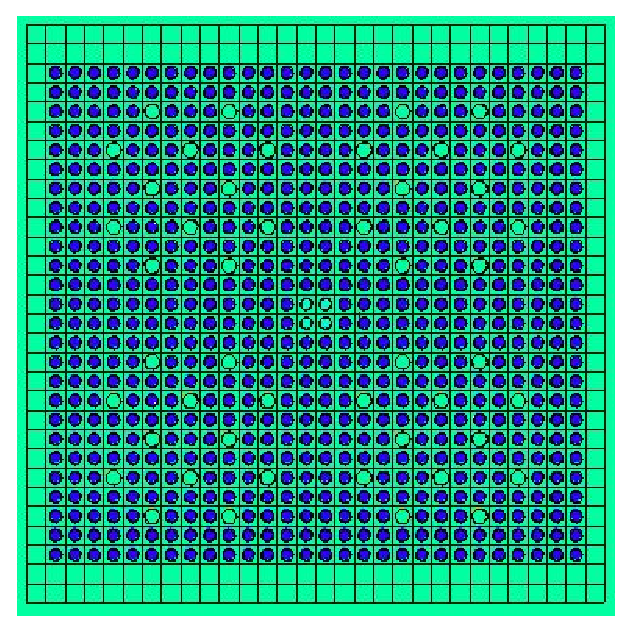
\includegraphics[scale=0.5]{LaTeX/Figures/Reactor-(Th-U)}
	\end{center}
\end{figure}

\begin{figure}[htpb]
	\caption{\label{cross} Arranjo em cruz para as varetas de teste.}
	\begin{center}
	    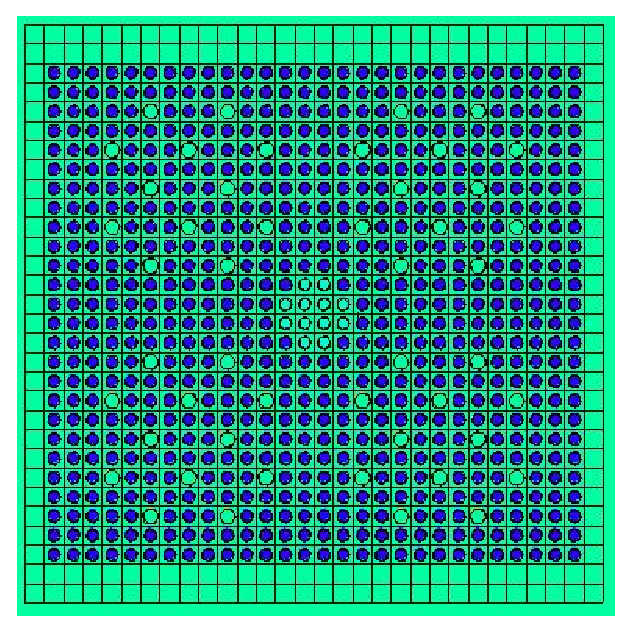
\includegraphics[scale=0.5]{LaTeX/Figures/Reactor-Th-Puro}
	\end{center}
\end{figure}

Em termos do código MCNP, são utilizado os comandos ``latt'' e ``fill'', que criam um espaço tridimensional de um tamanho definido e preenchem com universos criados utilizando o comando ``u'', este comando pode ser executado somente quando todos os universos tem o mesmo tamanho entre si e cabem dentro do espaço criado, o código que modela o núcleo do reator pode ser visto a seguir na configuração cruz:

\newpage
\begin{lstlisting}
c  Matrix plate   
c 
ccccccccccccccccccccccccccccccccccccc 
c 
24     4   1.00104E-01 -17  18  -19  20 lat=1  fill=-15:14 -15:14 0:0  
c      a b                                                     a b     
c      a a a b c d e f g h i j k l m n o p q r s t u v w x u z z z 
c                                                   ------------->
       7 7 7 7 7 7 7 7 7 7 7 7 7 7 7 7 7 7 7 7 7 7 7 7 7 7 7 7 7 7  $ ^ 29
       7 7 7 7 7 7 7 7 7 7 7 7 7 7 7 7 7 7 7 7 7 7 7 7 7 7 7 7 7 7  $ | 28
       7 1 1 1 1 1 1 1 1 1 1 1 1 1 1 1 1 1 1 1 1 1 1 1 1 1 1 1 1 7  $ | 27
       7 1 1 1 1 1 1 1 1 1 1 1 1 1 1 1 1 1 1 1 1 1 1 1 1 1 1 1 1 7  $ | 26
       7 1 1 1 1 1 3 1 1 1 3 1 1 1 1 1 1 1 1 4 1 1 1 4 1 1 1 1 1 7  $ | 25
       7 1 1 1 1 1 1 1 1 1 1 1 1 1 1 1 1 1 1 1 1 1 1 1 1 1 1 1 1 7  $ | 24
       7 1 1 1 3 1 1 1 3 1 1 1 3 1 1 1 1 4 1 1 1 4 1 1 1 4 1 1 1 7  $ | 23
       7 1 1 1 1 1 1 1 1 1 1 1 1 1 1 1 1 1 1 1 1 1 1 1 1 1 1 1 1 7  $   22
       7 1 1 1 1 1 3 1 1 1 3 1 1 1 1 1 1 1 1 4 1 1 1 4 1 1 1 1 1 7  $   21
       7 1 1 1 1 1 1 1 1 1 1 1 1 1 1 1 1 1 1 1 1 1 1 1 1 1 1 1 1 7  $   20
       7 1 1 1 3 1 1 1 3 1 1 1 3 1 1 1 1 4 1 1 1 4 1 1 1 4 1 1 1 7  $   19
       7 1 1 1 1 1 1 1 1 1 1 1 1 1 1 1 1 1 1 1 1 1 1 1 1 1 1 1 1 7  $   18
       7 1 1 1 1 1 3 1 1 1 3 1 1 1 1 1 1 1 1 4 1 1 1 4 1 1 1 1 1 7  $   17
       7 1 1 1 1 1 1 1 1 1 1 1 1 1 9 9 1 1 1 1 1 1 1 1 1 1 1 1 1 7  $   16
       7 1 1 1 1 1 1 1 1 1 1 1 1 9 9 9 9 1 1 1 1 1 1 1 1 1 1 1 1 7  $   15
       7 1 1 1 1 1 1 1 1 1 1 1 1 9 9 9 9 1 1 1 1 1 1 1 1 1 1 1 1 7  $   14
       7 1 1 1 1 1 1 1 1 1 1 1 1 1 9 9 1 1 1 1 1 1 1 1 1 1 1 1 1 7  $   13
       7 1 1 1 1 1 4 1 1 1 4 1 1 1 1 1 1 1 1 3 1 1 1 3 1 1 1 1 1 7  $   12
       7 1 1 1 1 1 1 1 1 1 1 1 1 1 1 1 1 1 1 1 1 1 1 1 1 1 1 1 1 7  $   11
       7 1 1 1 4 1 1 1 4 1 1 1 4 1 1 1 1 3 1 1 1 3 1 1 1 3 1 1 1 7  $   10
       7 1 1 1 1 1 1 1 1 1 1 1 1 1 1 1 1 1 1 1 1 1 1 1 1 1 1 1 1 7  $   09
       7 1 1 1 1 1 4 1 1 1 4 1 1 1 1 1 1 1 1 3 1 1 1 3 1 1 1 1 1 7  $   08
       7 1 1 1 1 1 1 1 1 1 1 1 1 1 1 1 1 1 1 1 1 1 1 1 1 1 1 1 1 7  $   07
       7 1 1 1 4 1 1 1 4 1 1 1 4 1 1 1 1 3 1 1 1 3 1 1 1 3 1 1 1 7  $   06
       7 1 1 1 1 1 1 1 1 1 1 1 1 1 1 1 1 1 1 1 1 1 1 1 1 1 1 1 1 7  $   05
       7 1 1 1 1 1 4 1 1 1 4 1 1 1 1 1 1 1 1 3 1 1 1 3 1 1 1 1 1 7  $   04
       7 1 1 1 1 1 1 1 1 1 1 1 1 1 1 1 1 1 1 1 1 1 1 1 1 1 1 1 1 7  $   03
       7 1 1 1 1 1 1 1 1 1 1 1 1 1 1 1 1 1 1 1 1 1 1 1 1 1 1 1 1 7  $   02
       7 7 7 7 7 7 7 7 7 7 7 7 7 7 7 7 7 7 7 7 7 7 7 7 7 7 7 7 7 7  $   01
       7 7 7 7 7 7 7 7 7 7 7 7 7 7 7 7 7 7 7 7 7 7 7 7 7 7 7 7 7 7  $   00
       imp:n=1
       u=7
\end{lstlisting}

Os universos utilizados na matriz são definidos da seguitne forma:
\begin{itemize}
\item u=1: Varetas combustíveis comuns, urânio enriquecido a 5\%;
\item u=2: Barras de Controle;
\item u=3: Tubos guia das Barras de Controle;
\item u=4: Tubos guia das Barras de Segurança;
\item u=5: Barras de Segurança;
\item u=9: Varetas de ensaio;
\end{itemize}
A variação do arranjo, também prevista por MOREIRA, ocorre em virtude
da natureza fértil (e não físsil) do Tório, altas concentrações de
Tório no nucleo do reator causam uma queda no fator k e podem, se
mal dimensionadas, causar o interrompimento da reação em cadeia em
médio prazo, por isso é ideal utilizar menos varetas caso haja muito
Tório por vareta, o arranjo ideal é aquele que mantém o valor de k
levemente acima de 1 sem adição excessiva de Boro ou inserção das
barras de controle.

\section{Aproximações Consideradas}

Como ja foi abordado na introdução deste trabalho, os resultados fornecidos pelo MCNP dependem de diversos fatores governados pelos dados do arquivo \textit{input, }enquanto os parâmetros de composição das varetas ja foram abordados por MOREIRA,  outros parâmetros, necessários para a execução do código, são baseados em sugestões abordadas manual do programa MCNPX.

\subsection{Parâmetros de Condições iniciais}

O código do MCNP exige que sejam fornecidos nêutrons primordiais para que sejam feitas as primeiras iterações da simulação através dos cartões de fonte, a utilização de nêutrons pontuais torna mais lento o processo de convergência, para contornar esta limitação foi utilizada a função de distribuição inicial de nêutrons em um cilindro de 54,84cm de altura e 16,5cm de raio localizado no centro do reator (posição 0 0 0) e orientado no eixo Y, o código utilizado nos cartões de fonte pode ser observado a seguir.

\begin{lstlisting}
c  SOURCE CARDS 
c  
sdef    pos= 0 0 0     $ center of volume source          
        axs= 0 0 1     $ axis of volume source (cylinder)          
        rad d1         $ radial bins to define by distributions 1          
        ext d2         $ axial bins to define by distributions 2          
        erg d3         $ energy distributions defined by distr. 3  
si1     h 0 16.5       $ radii of volume source  
si2     h -27.42 27.42 $ extension of cylinder (+/-) from the center  
sp3    -3              $ built in function: Watt fission spectrum
\end{lstlisting}

\newpage
\subsection{Parâmetros de Ensaio}

Para os ensaios realizados foram utilizados sempre os mesmos parâmetros,
o cartão kcode utilizado poe ser observado a seguir:

\begin{lstlisting}
kcode  200000 1.02 20 1000
\end{lstlisting}

Na sequência em que são inseridos le-se:
\begin{itemize}
\item nsrck = 200000: Foram simulados sempre duzendos mil nêutrons a cada
ciclo de simulação;
\item rkk = 1.02: O $k_{ef}$ do reator em t=0 foi de 1.020;
\item izk = 20: Os dados referentes aos 20 primeiros ciclos de simulação
foram descartado;
\item kct: = 1000: Foram simulados 1000 ciclos no total, ou seja, 980 ciclos
de aquisição de dados.
\end{itemize}

% ----------------------------------------------------------
% PARTE
% ----------------------------------------------------------
\part*{Resultados}
% ----------------------------------------------------------

Após 1000 ciclos de simulação foram obtidos os dados de k do reator,
os resultados podem ser observados nas tabelas\ref{cross68} a\ref{2x2_99} abaixo:


\begin{center}
\begin{longtable}{|l|l|l|}
\caption[Resultados de $k_{ef}$ para as composições Th-U no arranjo em cruz, confiança de 68\%;]{Resultados de $k_{ef}$ para as composições Th-U no arranjo em cruz, confiança de 68\%}
\label{cross68} \\
% header ------------------------
\hline 
Composição da Vareta & $k_{ef}$ & $\sigma$\tabularnewline
\hline 
\hline 
$ThO_{2}$ puro & 0,98962 & $0,0005$ \tabularnewline
\hline 
 $(75\%Th-25\%U)O_{2}$ & 0,99693 & $0,0005$ \tabularnewline
\hline 
 $(50\%Th-20\%U)O_{2}$ & 1,00457 & $0,0005$ \tabularnewline
\hline 
\end{longtable}

\begin{longtable}{|l|l|l|}
\caption[Resultados de $k_{ef}$ para as composições Th-U no arranjo 2x2, confiança de 68\%;]{Resultados de $k_{ef}$ para as composições Th-U no arranjo 2x2, confiança de 68\%}
\label{2x2_68} \\
% header ------------------------
\hline 
Composição da Vareta & $k_{ef}$ & $\sigma$\tabularnewline
\hline 
\hline 
$ThO_{2}$ puro & 0,98962 & $0,00005$ \tabularnewline
\hline 
 $(75\%Th-25\%U)O_{2}$ & 0,99693 & $0,00005$ \tabularnewline
\hline 
 $(50\%Th-20\%U)O_{2}$ & 1,00457 & $0,00005$ \tabularnewline
\hline 
\end{longtable}

\begin{longtable}{|l|l|l|}
\caption[Resultados de $k_{ef}$ para as composições Th-U no arranjo em cruz, confiança de 95\%;]{Resultados de $k_{ef}$ para as composições Th-U no arranjo em cruz, confiança de 95\%;}
\label{cross95} \\
% header ------------------------
\hline 
Composição da Vareta & $k_{ef}$ & $\sigma$\tabularnewline
\hline 
\hline 
$ThO_{2}$ puro & 0,98962 & $0,00010$ \tabularnewline
\hline 
 $(75\%Th-25\%U)O_{2}$ & 0,99693 & $0,00010$ \tabularnewline
\hline 
 $(50\%Th-20\%U)O_{2}$ & 1,00457 & $0,00010$ \tabularnewline
\hline 
\end{longtable}

\begin{longtable}{|l|l|l|}
\caption[Resultados de $k_{ef}$ para as composições Th-U no arranjo 2x2, confiança de 95\%;]{Resultados de $k_{ef}$ para as composições Th-U no arranjo 2x2, confiança de 95\%;}
\label{2x2_95} \\
% header ------------------------
\hline 
Composição da Vareta & $k_{ef}$ & $\sigma$\tabularnewline
\hline 
\hline 
$ThO_{2}$ puro & 0,98962 & $0,00010$ \tabularnewline
\hline 
 $(75\%Th-25\%U)O_{2}$ & 0,99693 & $0,00010$ \tabularnewline
\hline 
 $(50\%Th-20\%U)O_{2}$ & 1,00457 & $0,00010$ \tabularnewline
\hline 
\end{longtable}

\newpage
\begin{longtable}{|l|l|l|}
\caption[Resultados de $k_{ef}$ para as composições Th-U no arranjo em cruz, confiança de 99\%;]{Resultados de $k_{ef}$ para as composições Th-U no arranjo em cruz, confiança de 99\%;}
\label{cross99} \\
% header ------------------------
\hline 
Composição da Vareta & $k_{ef}$ & $\sigma$\tabularnewline
\hline 
\hline 
$ThO_{2}$ puro & 0,98962 & $0,00014$ \tabularnewline
\hline 
 $(75\%Th-25\%U)O_{2}$ & 0,99693 & $0,00013$ \tabularnewline
\hline 
 $(50\%Th-20\%U)O_{2}$ & 1,00457 & $0,00013$ \tabularnewline
\hline 
\end{longtable}

\begin{longtable}{|l|l|l|}
\caption[Resultados de $k_{ef}$ para as composições Th-U no arranjo 2x2, confiança de 99\%;]{Resultados de $k_{ef}$ para as composições Th-U no arranjo 2x2, confiança de 99\%;}
\label{2x2_99} \\
% header ------------------------
\hline 
Composição da Vareta & $k_{ef}$ & $\sigma$\tabularnewline
\hline 
\hline 
$ThO_{2}$ puro & 1,01010 & $0,00014$ \tabularnewline
\hline 
 $(75\%Th-25\%U)O_{2}$ & 1,01281 & $0,00013$ \tabularnewline
\hline 
 $(50\%Th-20\%U)O_{2}$ & 1,01577 & $0,00013$ \tabularnewline
\hline 
\end{longtable}

\end{center}

Existem algumas observações interessantes que podem ser feitas observando os dados obtidos nas simulações, uma delas é que fica extremamente clara a queda no fator de multiplicação induzida pela inserção do Tório no nucleo do reator. O maior valor obtido para k é de $1,01577$, este valor corresponde ao arranjo 2x2 com varetas que contém 50\% de Óxido de Urânio enriquecido e 50\% Óxido de Tório; ou seja, a configuração que insere a menor quantidade de Tório no reator e o menor valor de k obtido foi de $0,98962$ e é o correspondente ao arranjo em cruz com varetas que contém Óxido de Tório puro. Na secçao 1.2 do trabalho foie efeito era esperado devido ao fato de serem consumidos dois nêutrons para fissionar o Tório, um para a transmutação e o outro para a fissão.

Note que em Monte Carlo não sabemos qual é o valor médio, ele é estimado. Logo, a variância estabelece que temos um certo nível de segurança (de 99\%) que o valor médio esteja ente  $\pm$3 sigma, não que o valor esperado do experimento esteja dentro do intervalo. Conforme aumentamos a confiança da medição, ou seja, reduzimos a faixa observada na dispersão de Gauss, o valor de variância não aumenta significativamente; sempre se mantém em menos de 0,02\% do valor total. Isto aponta para uma Gaussiana com perfil agudo, ou seja, os dados tem alto grau de convergência. Outro detalhe é que a incerteza (variância) diminuí com o inverso da raiz do número de histórias, logo, para diminuirmos a variância pela metade teríamos que quadruplicar o número de histórias, ou seja, quadruplicar o tempo de cálculo.
% ----------------------------------------------------------
% Finaliza a parte no bookmark do PDF
% para que se inicie o bookmark na raiz
% e adiciona espaço de parte no Sumário
% ----------------------------------------------------------
\phantompart

% ---
% Conclusão
% ---
\chapter{Conclusão}
% ---

O objetivo deste trabalho era desenvolver uma base de comparação para os dados nucleares do Tório, utilizando as tabelas do MCNP, com a finalidade de propor um experimento real no reator IPEN/MB-01. Obviamente, varias configurações são possíveis mas, dentro da proposta apresentada, observando os dados, vemos que a melhor configuração irá depender de quão oneroso será o processo de produção das varetas de teste. 

Os dados coletados são bastante conclusivos, a variância de 0,00014 considerando 99\% de confiança está em patamares excelentes, não há motivos para acreditar que a comparação de dados reais com os dados dessa simulação possa gerar quaisquer discrepâncias.  De um ponto de vista prático, os valores menores de k, observados nas simulações com o arranjo em cruz, apontam para uma menor utilização de barras de controle, o que levaria a uma menor interferência na análise dos dados de secção de choque do Tório, entretanto, a utilização de um menor número de barras no arranjo 2x2 não impossibilida o estudo e é uma estratégia válida caso o proce/sso de manufatura das varetas seja um gargalo na execução do ensaio. Dito isso é importante relatar que está prevista uma atualização no núcleo do IPEN/MB-01, desconhecida durante o desenvolvimento deste trabalho, o novo núcleo do reator utilizará um arranjo de placas radicalmente diferente do núcleo simulado. Este fato não invalida completamente o experimento, ainda que não possa ser dado prosseguimento da forma que foi planejada no início do trabalho, a análise dos resultados aponta que a equipe envolvida nas simulações é competente para simular o novo núcleo do reator para um ensaio real nesta nova configuração.

Os dados nucleares, de uma forma geral, estão em constante reavaliação, como é sempre necessário com dados empíricos. Como já foi citado na introdução deste trabalho, a verificação dos dados do Tório é etapa fundamental do desenvolvimento de reatores capazes de queimar este elemento e este trabalho pode servir como base para futuros estudos similares. No intuito de facilitar o desenvolvimento do \emph{input} para o MCNPX e, por ventura um texto em LaTeX, todos os dados de desenvolvimento deste trabalho estão comentados e disponíveis na íntegra através do endereço <https://github.com/LFBianchi/MB-01-MCNPX-ToriumRods>.

% ----------------------------------------------------------
% ELEMENTOS PÓS-TEXTUAIS
% ----------------------------------------------------------
\postextual
% ----------------------------------------------------------

% ----------------------------------------------------------
% Referências bibliográficas
% ----------------------------------------------------------
\bibliography{LUIZ_SANTOS_11101610-Ref}

% ----------------------------------------------------------
% Glossário
% ----------------------------------------------------------
%
% Consulte o manual da classe abntex2 para orientações sobre o glossário.
%
%\glossary
0
8*/-
% ----------------------------------------------------------
% Apêndices
% ----------------------------------------------------------

% ---
% Inicia os apêndices
% ---
\begin{apendicesenv}

% Imprime uma página indicando o início dos apêndices
\partapendices

% ----------------------------------------------------------
\chapter{Código Base da Simulação para a IPEN/MB-01 em Configuração Padrão}
% ----------------------------------------------------------

\begin{lstlisting}
Critical Facility  4.3 w/o u-235 enrichment
c ccccccccccccccccccccccccccccccccccccc
c  Fuel Rod 
c ccccccccccccccccccccccccccccccccccccc
c
c  UO2 pellets
c
1  1    6.813709e-02
        (-1 3 -2)
        imp:n=1
        u=1
c
c  aluminum stopple up
c
2  5    1.118600e-01
        (-5 2 -4)
        imp:n=1
        u=1
c
c  aluminum stopple botton
c
3  5    1.118600e-01
        (-5 -3)
        imp:n=1
        u=1
c
c Spacer Tube
c 
4  7    8.802220E-02
        (4 -7 6) 
        imp:n=1
        u=1
c
c Gap 
c
5 2     -1.20492E-3
        (5 -7  2 -4 ):   $ gap top 
        (5 -7 -3    ):   $ gap botton
        (3 -2  1 -7 ):   $ gap U02
        (7 -9       )    $ gap    
        imp:n=1
        u=1
c
c Void 
c
6  0 
        (-6 4) 
        imp:n=1
        u=1
c
c Cladding
c
7  3    8.655893e-02
        (9 -10)
        imp:n=1
        u=1
c
c Water 
c 
8  4    1.00104E-01
        (10)
        imp:n=1
        u=1
c
c ccccccccccccccccccccccccccccccccccccc
c  Control-Rod  
c ccccccccccccccccccccccccccccccccccccc
c
c Absorber
c
9    6  5.8233510e-02
        (-13 12)
        imp:n=1
        u=2
c
c Gap 
c
10   2  -1.20492E-3
        (13 -9 12) $ gap
        imp:n=1
        u=2
c
c Tip and Cladding
c
11   3  8.655893e-02
        (9  -10  12):
        (11 -12 -10)
        imp:n=1
        u=2
c
c Water 
c 
12  4   1.00104E-01 
        ( 10    ):
        (-10 -11)
        imp:n=1
        u=2
c
c ccccccccccccccccccccccccccccccccccccc
c  Guide tube plus Control-Rod  
c ccccccccccccccccccccccccccccccccccccc
c
c  Control-Rod region
c
13  0   (-14) 
        fill=2 (0 0 0)
        imp:n=1
        u=3
c
c  Guide tube 
c
14  9   8.429047E-02
        (14 -15)
        imp:n=1
        u=3
c
c Water 
c 
15  4   1.00104E-01
        (15)
        imp:n=1
        u=3
c
c ccccccccccccccccccccccccccccccccccccc
c  Safety-rod guide tube 
c ccccccccccccccccccccccccccccccccccccc
c
c Water 
c 
16  4   1.00104E-01
        (-14) 
        imp:n=1
        u=4
c
c  Guide tube 
c
17  9   8.429047E-02
        (14 -15)
        imp:n=1
        u=4
c
c Water 
c 
18  4   1.00104E-01
        (15)
        imp:n=1
        u=4
c
c ccccccccccccccccccccccccccccccccccccc
c  Gd2O3 
c ccccccccccccccccccccccccccccccccccccc
c
c Gd2O3
c
19  13  1.7167297e-02
        (-9)
        imp:n=1
        u=5
c
c Cladding
c
20  3   8.655893e-02
        (9 -10)
        imp:n=1
        u=5
c
c Water 
c 
21  4   1.00104E-01
        (10)
        imp:n=1
        u=5
c
c ccccccccccccccccccccccccccccccccccccc
c  Stainless Steel rod  
c ccccccccccccccccccccccccccccccccccccc
c
c Steel
c
22  8   8.216686e-02
        (-16)
        imp:n=1
        u=6
c
c Water 
c 
23  4   1.00104E-01
        (16)
        imp:n=1
        u=6
c
c ccccccccccccccccccccccccccccccccccccc
c  Matrix plate  
c ccccccccccccccccccccccccccccccccccccc
c
24     4   1.00104E-01 -17  18  -19  20 lat=1  fill=-15:14 -15:14 0:0 
c      a b                                                     a b    
c      a a a b c d e f g h i j k l m n o p q r s t u v w x u z z z
c                                                   -------------> 
       7 7 7 7 7 7 7 7 7 7 7 7 7 7 7 7 7 7 7 7 7 7 7 7 7 7 7 7 7 7  $ ^ 29    
       7 7 7 7 7 7 7 7 7 7 7 7 7 7 7 7 7 7 7 7 7 7 7 7 7 7 7 7 7 7  $ | 28    
       7 1 1 1 1 1 1 1 1 1 1 1 1 1 1 1 1 1 1 1 1 1 1 1 1 1 1 1 1 7  $ | 27    
       7 1 1 1 1 1 1 1 1 1 1 1 1 1 1 1 1 1 1 1 1 1 1 1 1 1 1 1 1 7  $ | 26    
       7 1 1 1 1 1 3 1 1 1 3 1 1 1 1 1 1 1 1 4 1 1 1 4 1 1 1 1 1 7  $ | 25    
       7 1 1 1 1 1 1 1 1 1 1 1 1 1 1 1 1 1 1 1 1 1 1 1 1 1 1 1 1 7  $ | 24    
       7 1 1 1 3 1 1 1 3 1 1 1 3 1 1 1 1 4 1 1 1 4 1 1 1 4 1 1 1 7  $ | 23    
       7 1 1 1 1 1 1 1 1 1 1 1 1 1 1 1 1 1 1 1 1 1 1 1 1 1 1 1 1 7  $   22    
       7 1 1 1 1 1 3 1 1 1 3 1 1 1 1 1 1 1 1 4 1 1 1 4 1 1 1 1 1 7  $   21    
       7 1 1 1 1 1 1 1 1 1 1 1 1 1 1 1 1 1 1 1 1 1 1 1 1 1 1 1 1 7  $   20    
       7 1 1 1 3 1 1 1 3 1 1 1 3 1 1 1 1 4 1 1 1 4 1 1 1 4 1 1 1 7  $   19    
       7 1 1 1 1 1 1 1 1 1 1 1 1 1 1 1 1 1 1 1 1 1 1 1 1 1 1 1 1 7  $   18    
       7 1 1 1 1 1 3 1 1 1 3 1 1 1 1 1 1 1 1 4 1 1 1 4 1 1 1 1 1 7  $   17    
       7 1 1 1 1 1 1 1 1 1 1 1 1 1 1 1 1 1 1 1 1 1 1 1 1 1 1 1 1 7  $   16    
       7 1 1 1 1 1 1 1 1 1 1 1 1 1 1 1 1 1 1 1 1 1 1 1 1 1 1 1 1 7  $   15    
       7 1 1 1 1 1 1 1 1 1 1 1 1 1 1 1 1 1 1 1 1 1 1 1 1 1 1 1 1 7  $   14    
       7 1 1 1 1 1 1 1 1 1 1 1 1 1 1 1 1 1 1 1 1 1 1 1 1 1 1 1 1 7  $   13    
       7 1 1 1 1 1 4 1 1 1 4 1 1 1 1 1 1 1 1 3 1 1 1 3 1 1 1 1 1 7  $   12    
       7 1 1 1 1 1 1 1 1 1 1 1 1 1 1 1 1 1 1 1 1 1 1 1 1 1 1 1 1 7  $   11    
       7 1 1 1 4 1 1 1 4 1 1 1 4 1 1 1 1 3 1 1 1 3 1 1 1 3 1 1 1 7  $   10    
       7 1 1 1 1 1 1 1 1 1 1 1 1 1 1 1 1 1 1 1 1 1 1 1 1 1 1 1 1 7  $   09    
       7 1 1 1 1 1 4 1 1 1 4 1 1 1 1 1 1 1 1 3 1 1 1 3 1 1 1 1 1 7  $   08    
       7 1 1 1 1 1 1 1 1 1 1 1 1 1 1 1 1 1 1 1 1 1 1 1 1 1 1 1 1 7  $   07    
       7 1 1 1 4 1 1 1 4 1 1 1 4 1 1 1 1 3 1 1 1 3 1 1 1 3 1 1 1 7  $   06    
       7 1 1 1 1 1 1 1 1 1 1 1 1 1 1 1 1 1 1 1 1 1 1 1 1 1 1 1 1 7  $   05    
       7 1 1 1 1 1 4 1 1 1 4 1 1 1 1 1 1 1 1 3 1 1 1 3 1 1 1 1 1 7  $   04    
       7 1 1 1 1 1 1 1 1 1 1 1 1 1 1 1 1 1 1 1 1 1 1 1 1 1 1 1 1 7  $   03    
       7 1 1 1 1 1 1 1 1 1 1 1 1 1 1 1 1 1 1 1 1 1 1 1 1 1 1 1 1 7  $   02    
       7 7 7 7 7 7 7 7 7 7 7 7 7 7 7 7 7 7 7 7 7 7 7 7 7 7 7 7 7 7  $   01     
       7 7 7 7 7 7 7 7 7 7 7 7 7 7 7 7 7 7 7 7 7 7 7 7 7 7 7 7 7 7  $   00       
       imp:n=1
       u=7
c
c Lattice region 
c
25 0 
       (22 -21 24 -23 26 -25) 
       fill=7 (0.75 0.75 0)
       imp:n=1
       u=8
c
c bottom grid plate
c
26 12  8.666089e-02
       (28 -27 30 -29 -26 31)
       imp:n=1
       u=8
c
c Water 
c 
28 4   1.00104E-01
       (-31               ):
       (31 -26  27        ):
       (31 -26 -28        ):
       (31 -26 -27 28 29  ):
       (31 -26 -27 28 -30 ): 
       (26 -25  21        ):
       (26 -25 -22        ):
       (26 -25 -21 22  23 ):
       (26 -25 -21 22 -24 ):
       (25                )
       imp:n=1
       u=8
c
c cccccccccccccccccccccccccc
c
c System 
c 
29     0  
       (37 -38 -39) fill=8
       imp:n=1
c
c Outside
c
999    0  
       (39):
       (-39 38):
       (-39 -37)
       imp:n=0
c
c ccccccccccccccccccccccccccccccccccccccccccccccccccccccccccccccccccccccc
 
c ccccccccccccccccccccccccccccccccccccccccccccccccccccccccccccccccccccccc
c
1    cz   0.42447   $  UO2 : OR
2    pz  27.42    $ --| - (+) -> 54.84             
3    pz -27.42    $ --|
c
4    pz  32.82     $   
5    cz  0.4235    $  Al2O3 : OR
c
6    cz  0.365    $ Spacer Tube : IR
7    cz  0.425    $ Spacer Tube : OR
c
9    cz  0.42873  $ Cladding : IR
10   cz  0.49037  $ Cladding : OR
c
c
11   pz  25.75   $
12   pz  27.42   $
13   cz  0.416   $ Ag-In-Cd : OR
c
14   cz  0.565   $ Guide Tube : IR
15   cz  0.6     $ Guide Tube : OR
c
16   cz 0.475    $ Stainless Steel rod : OR 
c
17   px  0.75000 $ half pitch 
18   px -0.75000 $ half pitch
19   py  0.75000 $ half pitch
20   py -0.75000 $ half pitch
c
21   px  22.5
22   px -22.5  
23   py  22.5
24   py -22.5
c
25   pz  43.78 
26   pz -36.52
c
27   px   29.4  $ bottom grid plate +X
28   px  -29.4  $ bottom grid plate -X
29   py   29.4  $ bottom grid plate +Y
30   py  -29.4  $ bottom grid plate -Y
c
31   pz  -38.72
c
32   px -28.5   $ steel plate (ref. sur 22)
c
33   py  25.4
34   py -25.4
c
35   pz  39.13
36   pz -32.37
c
37   pz -88.72 $ reactor tank botton
38   pz  93.78 $ reactor tank top
c
39   cz 100.00  $ reactor tank radius
c
c ccccccccccccccccccccccccccccccccccccccccccccccccccccccccccccccccccccccc

c ccccccccccccccccccccccccccccccccccccccccccccccccccccccccccccccccccccccc
c
c  SOURCE CARDS
c
 sdef    pos= 0 0 0     $ center of volume source
         axs= 0 0 1     $ axis of volume source (cylinder)
         rad d1         $ radial bins to define by distributions 1
         ext d2         $ axial bins to define by distributions 2
         erg d3         $ energy distributions defined by distr. 3
 si1     h 0 16.5       $ radii of volume source
 si2     h -27.42 27.42 $ extension of cylinder (+/-) from the center
 sp3    -3              $ built in function: Watt fission spectrum
c 
kcode  200000 1.02 20 1000
c
c ccccccccccccccccccccccccccccccccccccc
c  Material Definitions 
c ccccccccccccccccccccccccccccccccccccc
c
c   UO2 pellet 
c
m1   92234.50c 7.84560e-06 
     92235.50c 9.99160e-04 
     92238.50c 2.16920e-02 
      8016.50c 4.54677e-02
      8017.60c 1.72843e-05
c
c   AIR - 1.20492E-3 g/cm^3
c
 m2   GAS=1
      7014  7.81524E-01
      7015  2.87090E-03
      8016  2.10651E-01
      8017  8.00776E-05
      6000  1.60708E-04
      18000 4.71299E-03
c
c   SS304 clad - clad
c
m3    6000.50c 1.12390e-04 
     14000.50c 6.79340e-04 
     15031.50c 4.00400e-05
     16000.60c 1.56170e-05 
     24000.50c 1.68240e-02
     25055.50c 1.46450e-03 
     26000.55c 5.90020e-02 
     27059.50c 1.74020e-04
     28000.50c 8.16250e-03 
     42000.50c 8.45200e-05
c
c    H2O - water
c
m4    1001.50c 6.67360e-02 
      8016.50c 3.33553e-02 
      8017.60c 1.26798e-05
mt4   lwtr.01t
c
c   al2o3 - Alumina
c
m5    8016.50c 6.70905e-02 
      8017.60c 2.55041e-05
     13027.50c 4.47440e-02 
c
c    AG-IN-CD Control ROD
c
m6     6000.50c 1.50520e-03 
       8016.50c 1.76963e-03 
       8017.60c 6.72714e-07
      16000.60c 1.87910e-04
      47107.50c 2.31790e-02 
      47109.50c 2.11460e-02
      48000.50c 2.58940e-03
      49000.60c 7.85170e-03 
c
c     spacer tube - SS304
c
m7     6000.50c 2.40780e-04 
      14000.50c 1.11550e-03 
      15031.50c 3.11240e-05
      24000.50c 1.67790e-02
      25055.50c 1.15810e-03 
      26000.55c 6.18920e-02 
      27059.50c 1.14500e-04
      28000.50c 6.57020e-03 
c
c    stainless steel reflector - baffle 
c
m8     6000.50c 1.80900e-04
      14000.50c 6.96440e-04
      16000.60c 1.08160E-05
      22000.50c 2.40980e-06
      24000.50c 1.75950e-02
      25055.50c 1.03920e-03 
      26000.55c 6.00360e-02
      28000.50c 6.56700e-03
      29000.50c 1.66790e-05 
      42000.50c 2.10910e-05 
c
c     guide tube - SS304 
c
m9     6000.50c 8.89680e-05
      14000.50c 6.61700e-04 
      15031.50c 4.50000e-05
      24000.50c 1.62980e-02
      25055.50c 1.15010e-03 
      26000.55c 5.69430e-02 
      28000.50c 9.10370e-03 
c
c      SS304 Bottom Grid Plate
c
m10    5010.60c 2.9974e-04 
       5011.60c 1.2065e-03 
       6000.60c 3.7656e-04
       8016.60c 5.7928e-02 
      11023.60c 8.6686e-06
      12000.60c 8.1995e-05
      13027.60c 3.8619e-02
      24000.50c 3.8327e-06
      26000.55c 1.0705e-05
      28000.50c 3.3956e-06 
      62149.50c 2.6508e-07
      72000.60c 2.2331e-07
c
c    acrylic tube
c
m11    1001.60c 5.68840e-02 
       6000.60c 3.55520e-02
       8016.60c 1.42210e-02 
c
c     bottom grid plate
c
m12    6000.50c 7.94260e-05
      14000.50c 8.66160e-04 
      15031.50c 5.54400e-05
      16000.60c 4.46200e-06 
      24000.50c 1.67050e-02
      25055.50c 1.25030e-03 
      26000.55c 6.00360e-02
      28000.50c 7.66410e-03 
      42000.50c 2.98310e-05
c
c     gd2o3 powder density = 2.0668 g/cm3 
c
m13    8016.50c 1.03091e-02
       8017.60c 3.91894e-06
      64152.50c 1.37512E-05 
      64154.50c 1.49888E-04
      64155.50c 1.01759E-03 
      64156.50c 1.40743E-03 
      64157.50c 1.07603E-03
      64158.50c 1.70790E-03 
      64160.60c 1.50300E-03 
c
c
prdmp 1j 100 -1
print
\end{lstlisting}

\end{apendicesenv}
% ---


% ----------------------------------------------------------
% Anexos
% ----------------------------------------------------------

% ---
% Inicia os anexos
% ---
\begin{anexosenv}

% Imprime uma página indicando o início dos anexos
\partanexos

% ----------------------------------------------------------
\chapter{Código para as Varetas de Ensaio}
% ----------------------------------------------------------
\begin{itemize}
\item Varetas de ensaio com Óxido de Tório puro.
\begin{lstlisting}
c ccccccccccccccccccccccccccccccccccccc
c  Thorium Rod 
c ccccccccccccccccccccccccccccccccccccc
c
c  Thorium pellets
c
101  14   6.9450e-02
        (-1 3 -2)
        imp:n=1
        u=9
c
c  aluminum stopple up
c
102  5    1.118600e-01
        (-5 2 -4)
        imp:n=1
        u=9
c
c  aluminum stopple botton
c
103  5    1.118600e-01
        (-5 -3)
        imp:n=1
        u=9
c
c Spacer Tube
c 
104  7    8.802220E-02
        (4 -7 6) 
        imp:n=1
        u=9
c
c Gap 
c
105 2     -1.20492E-3
        (5 -7  2 -4 ):   $ gap top 
        (5 -7 -3    ):   $ gap botton
        (3 -2  1 -7 ):   $ gap U02
        (7 -9       )    $ gap    
        imp:n=1
        u=9
c
c Void 
c
106  0 
        (-6 4) 
        imp:n=1
        u=9
c
c Cladding
c
107  3    8.655893e-02
        (9 -10)
        imp:n=1
        u=9
c
c Water 
c 
108  4    1.00104E-01
        (10)
        imp:n=1
        u=9
c
\end{lstlisting}

\item Varetas de ensaio com 25\% de Óxido de Urânio enriquecido (5\%) e 75\% Óxido de de Tório.
\begin{lstlisting}
c ccccccccccccccccccccccccccccccccccccc
c  Thorium Rod 
c ccccccccccccccccccccccccccccccccccccc
c
c  Thorium pellets
c
101  14   6.8693e-02
        (-1 3 -2)
        imp:n=1
        u=9
c
c  aluminum stopple up
c
102  5    1.118600e-01
        (-5 2 -4)
        imp:n=1
        u=9
c
c  aluminum stopple botton
c
103  5    1.118600e-01
        (-5 -3)
        imp:n=1
        u=9
c
c Spacer Tube
c 
104  7    8.802220E-02
        (4 -7 6) 
        imp:n=1
        u=9
c
c Gap 
c
105 2     -1.20492E-3
        (5 -7  2 -4 ):   $ gap top 
        (5 -7 -3    ):   $ gap botton
        (3 -2  1 -7 ):   $ gap U02
        (7 -9       )    $ gap    
        imp:n=1
        u=9
c
c Void 
c
106  0 
        (-6 4) 
        imp:n=1
        u=9
c
c Cladding
c
107  3    8.655893e-02
        (9 -10)
        imp:n=1
        u=9
c
c Water 
c 
108  4    1.00104E-01
        (10)
        imp:n=1
        u=9
c
\end{lstlisting}

\item Varetas de ensaio com 50\% de Óxido de Urânio enriquecido (5\%) e 50\% de Óxido de Tório.
\begin{lstlisting}
c ccccccccccccccccccccccccccccccccccccc
c  Thorium Rod 
c ccccccccccccccccccccccccccccccccccccc
c
c  Thorium pellets
c
101  14   6.8055e-02
        (-1 3 -2)
        imp:n=1
        u=9
c
c  aluminum stopple up
c
102  5    1.118600e-01
        (-5 2 -4)
        imp:n=1
        u=9
c
c  aluminum stopple botton
c
103  5    1.118600e-01
        (-5 -3)
        imp:n=1
        u=9
c
c Spacer Tube
c 
104  7    8.802220E-02
        (4 -7 6) 
        imp:n=1
        u=9
c
c Gap 
c
105 2     -1.20492E-3
        (5 -7  2 -4 ):   $ gap top 
        (5 -7 -3    ):   $ gap botton
        (3 -2  1 -7 ):   $ gap U02
        (7 -9       )    $ gap    
        imp:n=1
        u=9
c
c Void 
c
106  0 
        (-6 4) 
        imp:n=1
        u=9
c
c Cladding
c
107  3    8.655893e-02
        (9 -10)
        imp:n=1
        u=9
c
c Water 
c 
108  4    1.00104E-01
        (10)
        imp:n=1
        u=9
c
\end{lstlisting}
\end{itemize}

% ----------------------------------------------------------
\chapter{Código para os Arranjos de Varetas}
% ----------------------------------------------------------
\begin{itemize}
\item Código para o arranjo das varetas de teste em 2x2.
\begin{lstlisting}

c ccccccccccccccccccccccccccccccccccccc
c  Matrix plate  
c ccccccccccccccccccccccccccccccccccccc
c
24     4   1.00104E-01 -17  18  -19  20 lat=1  fill=-15:14 -15:14 0:0 
c      a b                                                     a b    
c      a a a b c d e f g h i j k l m n o p q r s t u v w x u z z z
c                                                   -------------> 
       7 7 7 7 7 7 7 7 7 7 7 7 7 7 7 7 7 7 7 7 7 7 7 7 7 7 7 7 7 7  $ ^ 29    
       7 7 7 7 7 7 7 7 7 7 7 7 7 7 7 7 7 7 7 7 7 7 7 7 7 7 7 7 7 7  $ | 28    
       7 1 1 1 1 1 1 1 1 1 1 1 1 1 1 1 1 1 1 1 1 1 1 1 1 1 1 1 1 7  $ | 27    
       7 1 1 1 1 1 1 1 1 1 1 1 1 1 1 1 1 1 1 1 1 1 1 1 1 1 1 1 1 7  $ | 26    
       7 1 1 1 1 1 3 1 1 1 3 1 1 1 1 1 1 1 1 4 1 1 1 4 1 1 1 1 1 7  $ | 25    
       7 1 1 1 1 1 1 1 1 1 1 1 1 1 1 1 1 1 1 1 1 1 1 1 1 1 1 1 1 7  $ | 24    
       7 1 1 1 3 1 1 1 3 1 1 1 3 1 1 1 1 4 1 1 1 4 1 1 1 4 1 1 1 7  $ | 23    
       7 1 1 1 1 1 1 1 1 1 1 1 1 1 1 1 1 1 1 1 1 1 1 1 1 1 1 1 1 7  $   22    
       7 1 1 1 1 1 3 1 1 1 3 1 1 1 1 1 1 1 1 4 1 1 1 4 1 1 1 1 1 7  $   21    
       7 1 1 1 1 1 1 1 1 1 1 1 1 1 1 1 1 1 1 1 1 1 1 1 1 1 1 1 1 7  $   20    
       7 1 1 1 3 1 1 1 3 1 1 1 3 1 1 1 1 4 1 1 1 4 1 1 1 4 1 1 1 7  $   19    
       7 1 1 1 1 1 1 1 1 1 1 1 1 1 1 1 1 1 1 1 1 1 1 1 1 1 1 1 1 7  $   18    
       7 1 1 1 1 1 3 1 1 1 3 1 1 1 1 1 1 1 1 4 1 1 1 4 1 1 1 1 1 7  $   17    
       7 1 1 1 1 1 1 1 1 1 1 1 1 1 1 1 1 1 1 1 1 1 1 1 1 1 1 1 1 7  $   16    
       7 1 1 1 1 1 1 1 1 1 1 1 1 1 9 9 1 1 1 1 1 1 1 1 1 1 1 1 1 7  $   15    
       7 1 1 1 1 1 1 1 1 1 1 1 1 1 9 9 1 1 1 1 1 1 1 1 1 1 1 1 1 7  $   14    
       7 1 1 1 1 1 1 1 1 1 1 1 1 1 1 1 1 1 1 1 1 1 1 1 1 1 1 1 1 7  $   13    
       7 1 1 1 1 1 4 1 1 1 4 1 1 1 1 1 1 1 1 3 1 1 1 3 1 1 1 1 1 7  $   12    
       7 1 1 1 1 1 1 1 1 1 1 1 1 1 1 1 1 1 1 1 1 1 1 1 1 1 1 1 1 7  $   11    
       7 1 1 1 4 1 1 1 4 1 1 1 4 1 1 1 1 3 1 1 1 3 1 1 1 3 1 1 1 7  $   10    
       7 1 1 1 1 1 1 1 1 1 1 1 1 1 1 1 1 1 1 1 1 1 1 1 1 1 1 1 1 7  $   09    
       7 1 1 1 1 1 4 1 1 1 4 1 1 1 1 1 1 1 1 3 1 1 1 3 1 1 1 1 1 7  $   08    
       7 1 1 1 1 1 1 1 1 1 1 1 1 1 1 1 1 1 1 1 1 1 1 1 1 1 1 1 1 7  $   07    
       7 1 1 1 4 1 1 1 4 1 1 1 4 1 1 1 1 3 1 1 1 3 1 1 1 3 1 1 1 7  $   06    
       7 1 1 1 1 1 1 1 1 1 1 1 1 1 1 1 1 1 1 1 1 1 1 1 1 1 1 1 1 7  $   05    
       7 1 1 1 1 1 4 1 1 1 4 1 1 1 1 1 1 1 1 3 1 1 1 3 1 1 1 1 1 7  $   04    
       7 1 1 1 1 1 1 1 1 1 1 1 1 1 1 1 1 1 1 1 1 1 1 1 1 1 1 1 1 7  $   03    
       7 1 1 1 1 1 1 1 1 1 1 1 1 1 1 1 1 1 1 1 1 1 1 1 1 1 1 1 1 7  $   02    
       7 7 7 7 7 7 7 7 7 7 7 7 7 7 7 7 7 7 7 7 7 7 7 7 7 7 7 7 7 7  $   01     
       7 7 7 7 7 7 7 7 7 7 7 7 7 7 7 7 7 7 7 7 7 7 7 7 7 7 7 7 7 7  $   00       
       imp:n=1
       u=7

\end{lstlisting}

\newpage
\item Código para o arranjo das varetas de teste em cruz.
\begin{lstlisting}

c ccccccccccccccccccccccccccccccccccccc
c  Matrix plate  
c ccccccccccccccccccccccccccccccccccccc
c
24     4   1.00104E-01 -17  18  -19  20 lat=1  fill=-15:14 -15:14 0:0 
c      a b                                                     a b    
c      a a a b c d e f g h i j k l m n o p q r s t u v w x u z z z
c                                                   -------------> 
       7 7 7 7 7 7 7 7 7 7 7 7 7 7 7 7 7 7 7 7 7 7 7 7 7 7 7 7 7 7  $ ^ 29    
       7 7 7 7 7 7 7 7 7 7 7 7 7 7 7 7 7 7 7 7 7 7 7 7 7 7 7 7 7 7  $ | 28    
       7 1 1 1 1 1 1 1 1 1 1 1 1 1 1 1 1 1 1 1 1 1 1 1 1 1 1 1 1 7  $ | 27    
       7 1 1 1 1 1 1 1 1 1 1 1 1 1 1 1 1 1 1 1 1 1 1 1 1 1 1 1 1 7  $ | 26    
       7 1 1 1 1 1 3 1 1 1 3 1 1 1 1 1 1 1 1 4 1 1 1 4 1 1 1 1 1 7  $ | 25    
       7 1 1 1 1 1 1 1 1 1 1 1 1 1 1 1 1 1 1 1 1 1 1 1 1 1 1 1 1 7  $ | 24    
       7 1 1 1 3 1 1 1 3 1 1 1 3 1 1 1 1 4 1 1 1 4 1 1 1 4 1 1 1 7  $ | 23    
       7 1 1 1 1 1 1 1 1 1 1 1 1 1 1 1 1 1 1 1 1 1 1 1 1 1 1 1 1 7  $   22    
       7 1 1 1 1 1 3 1 1 1 3 1 1 1 1 1 1 1 1 4 1 1 1 4 1 1 1 1 1 7  $   21    
       7 1 1 1 1 1 1 1 1 1 1 1 1 1 1 1 1 1 1 1 1 1 1 1 1 1 1 1 1 7  $   20    
       7 1 1 1 3 1 1 1 3 1 1 1 3 1 1 1 1 4 1 1 1 4 1 1 1 4 1 1 1 7  $   19    
       7 1 1 1 1 1 1 1 1 1 1 1 1 1 1 1 1 1 1 1 1 1 1 1 1 1 1 1 1 7  $   18    
       7 1 1 1 1 1 3 1 1 1 3 1 1 1 1 1 1 1 1 4 1 1 1 4 1 1 1 1 1 7  $   17    
       7 1 1 1 1 1 1 1 1 1 1 1 1 1 9 9 1 1 1 1 1 1 1 1 1 1 1 1 1 7  $   16    
       7 1 1 1 1 1 1 1 1 1 1 1 1 9 9 9 9 1 1 1 1 1 1 1 1 1 1 1 1 7  $   15    
       7 1 1 1 1 1 1 1 1 1 1 1 1 9 9 9 9 1 1 1 1 1 1 1 1 1 1 1 1 7  $   14    
       7 1 1 1 1 1 1 1 1 1 1 1 1 1 9 9 1 1 1 1 1 1 1 1 1 1 1 1 1 7  $   13    
       7 1 1 1 1 1 4 1 1 1 4 1 1 1 1 1 1 1 1 3 1 1 1 3 1 1 1 1 1 7  $   12    
       7 1 1 1 1 1 1 1 1 1 1 1 1 1 1 1 1 1 1 1 1 1 1 1 1 1 1 1 1 7  $   11    
       7 1 1 1 4 1 1 1 4 1 1 1 4 1 1 1 1 3 1 1 1 3 1 1 1 3 1 1 1 7  $   10    
       7 1 1 1 1 1 1 1 1 1 1 1 1 1 1 1 1 1 1 1 1 1 1 1 1 1 1 1 1 7  $   09    
       7 1 1 1 1 1 4 1 1 1 4 1 1 1 1 1 1 1 1 3 1 1 1 3 1 1 1 1 1 7  $   08    
       7 1 1 1 1 1 1 1 1 1 1 1 1 1 1 1 1 1 1 1 1 1 1 1 1 1 1 1 1 7  $   07    
       7 1 1 1 4 1 1 1 4 1 1 1 4 1 1 1 1 3 1 1 1 3 1 1 1 3 1 1 1 7  $   06    
       7 1 1 1 1 1 1 1 1 1 1 1 1 1 1 1 1 1 1 1 1 1 1 1 1 1 1 1 1 7  $   05    
       7 1 1 1 1 1 4 1 1 1 4 1 1 1 1 1 1 1 1 3 1 1 1 3 1 1 1 1 1 7  $   04    
       7 1 1 1 1 1 1 1 1 1 1 1 1 1 1 1 1 1 1 1 1 1 1 1 1 1 1 1 1 7  $   03    
       7 1 1 1 1 1 1 1 1 1 1 1 1 1 1 1 1 1 1 1 1 1 1 1 1 1 1 1 1 7  $   02    
       7 7 7 7 7 7 7 7 7 7 7 7 7 7 7 7 7 7 7 7 7 7 7 7 7 7 7 7 7 7  $   01     
       7 7 7 7 7 7 7 7 7 7 7 7 7 7 7 7 7 7 7 7 7 7 7 7 7 7 7 7 7 7  $   00       
       imp:n=1
       u=7
c

\end{lstlisting}
\end{itemize}
% ----------------------------------------------------------
\chapter{Cartões de Materiais Utilizados}
% ----------------------------------------------------------
\begin{itemize}
\item Cartão de materiais para as varetas com Óxido de Tório puro.
\begin{lstlisting}
c     Thorium pellet 
m14   90230.70c 2.3145e-02 
      90232.70c 4.6300e-06
       8016.70c 4.6189e-02
       8017.70c 1.8520e-05 
\end{lstlisting}

\item Cartão de materiais para as varetas com 25\% de Óxido de Urânio enriquecido (5\%) e 75\% Óxido de de Tório.
\begin{lstlisting}
c     Thorium pellet 
m14   90230.70c 1.7197e-02 
      90232.70c 3.4402e-06
      92238.70c 5.4469e-03 
      92235.70c 2.8668e-04
       8016.70c 4.5759e-02 
       8017.70c 1.8348e-05 
\end{lstlisting}

\item Cartão de materiais para as varetas com 50\% de Óxido de Urânio enriquecido (5\%) e 50\% de Óxido de Tório.
\begin{lstlisting}
c     Thorium pellet 
m14   90230.70c 1.1358e-02 
      90232.70c 2.2721e-06
      92238.70c 1.0793e-02 
      92235.70c 5.6803e-04
       8016.70c 4.5333e-02 
       8017.70c 1.8177e-05  
\end{lstlisting}
\end{itemize}

\end{anexosenv}
\end{document}
